%%%%%%%%%%%%%%%%%%%%%%%%%%%%%%%%%%%%%%%%%%%%%%%%%%%%%%%%%%%%%%%%%%%%%%%%%%
%%
%%	Author Submission: INFORMS Journal on Data Science (IJDS)
%%	Manuscript: IJDS-2026-0250.R1 (Substantially Revised Resubmission)
%%	Template: INFORMS-IJDS-Template.tex (informs4.cls, informs2014.bst)
%%
%%%%%%%%%%%%%%%%%%%%%%%%%%%%%%%%%%%%%%%%%%%%%%%%%%%%%%%%%%%%%%%%%%%%%%%%%%

\documentclass[ijds,dblanonrev]{informs4}

\usepackage[T1]{fontenc}
\usepackage{lmodern}
\usepackage{graphicx}
\graphicspath{{figures/}}
\usepackage{booktabs}
\usepackage{bm}
\usepackage{mathtools}
\usepackage{microtype}
\usepackage{enumerate}
\usepackage{url}
\usepackage{algorithm}
\usepackage{algpseudocode}
\usepackage{endnotes}

\OneAndAHalfSpacedXII % Current default line spacing for IJDS

% Natbib setup for INFORMS 2014 author-year style
\usepackage{natbib}
 \bibpunct[, ]{(}{)}{,}{a}{}{,}%
 \def\bibfont{\small}%
 \def\bibsep{\smallskipamount}%
 \def\bibhang{24pt}%
 \def\newblock{\ }%
 \def\BIBand{and}%

\EquationsNumberedThrough
\TheoremsNumberedThrough
\ECRepeatTheorems

\MANUSCRIPTNO{IJDS-2026-0250.R1}

\DeclareMathOperator{\Tr}{Tr}
\DeclareMathOperator{\diag}{diag}
\DeclareMathOperator{\vol}{vol}
\DeclareMathOperator{\rank}{rank}
\newcommand{\R}{\mathbb{R}}
\newcommand{\E}{\mathbb{E}}
\newcommand{\Scal}{\mathcal{S}}
\newcommand{\norm}[1]{\left\lVert#1\right\rVert}
\newcommand{\abs}[1]{\left\lvert#1\right\rvert}

\FUNDING{This research received no external commercial funding.}

\begin{document}

\RUNTITLE{Spectral Diagnostic Trajectories in Stochastic Service Systems}
\TITLE{Spectral Diagnostic Trajectories: Multi-Modal Hypergraph State-Space Tracking, Context Decoupling, and Congestion Mitigation in Stochastic Clinical Service Systems}

\ARTICLEAUTHORS{%
\AUTHOR{Blinded for Double-Anonymous Peer Review}
\AFF{Author identity withheld per journal double-anonymous review policy}
}

\RUNAUTHOR{Blinded for Peer Review}

\ABSTRACT{%
High-dimensional, multi-modal sequential decision processes in time-sensitive service networks---such as emergency healthcare facilities---experience severe performance degradation when underlying operational states undergo discrete regime shifts. Existing sequential data retrieval frameworks treat interactions as either memoryless queries or continuous manifold trajectories, failing to decouple obsolete context during sudden structural bifurcations and propagating queueing congestion across overloaded human servers. We develop Spectral Diagnostic Trajectories (SDT), a graph-theoretic methodology that models time-evolving multi-modal interaction states as dynamic hypergraphs spanning continuous physiological waveforms (projected via linear state-space Mamba models), discrete operational events, and unstructured clinical text. SDT tracks the algebraic connectivity (Fiedler value $\lambda_2$) of the normalized hypergraph Laplacian in linear time $\mathcal{O}(|E_t|)$ to detect state bifurcations, establishes formal context-leakage bounds using Chebyshev-filtered Cheeger bisections, and prefetches prospective records via constrained combinatorial knapsack optimization under cognitive surprisal limits. Across 9{,}000 simulated workflows evaluated on 1{,}000 standardized high-complexity encounters derived from MIMIC-IV and HiRID, SDT reduces time-to-correct-information by 28.9\% (62.97 vs.\ 88.52\,s) and raises decision accuracy to 93.9\% at a mean computational latency of 112.9\,ms. Integrating these individual savings into an $M/M/c$ Erlang C queueing network demonstrates that near-saturation service systems exhibit super-linear operational leverage, reducing expected customer waiting times by 12.3 minutes and eliminating over 10{,}200 hours of institutional boarding annually. The central insight of this work is that discrete topological cuts on spectral hypergraphs provide provably bounded context decoupling over continuous manifold smoothing in non-stationary decision processes, demonstrating how spectral data science algorithms directly relieve macro-level congestion in human-in-the-loop operational service networks.%
}

\KEYWORDS{dynamic hypergraphs, spectral graph theory, algebraic connectivity, context decoupling, Cheeger conductance, queueing systems, Erlang C congestion, healthcare operations research}

\maketitle

% =============================================================================
\section{Introduction}
\label{sec:introduction}

High-volume service environments such as hospital Emergency Departments (EDs) and Intensive Care Units (ICUs) operate as congested stochastic service systems where expert human agents face severe cognitive and temporal constraints. During an acute operational shift, an attending physician manages 20 to 30 concurrent, undifferentiated patients \citep{topol2019high,miotto2018deep}, each producing continuous streams of heterogeneous data spanning unstructured clinical narratives, discrete diagnostic codes, laboratory measurements, and high-frequency physiological waveforms sampled at up to 250\,Hz \citep{johnson2023mimic,hyland2020hirid}.

The critical bottleneck in these systems is not data availability, but information retrieval latency under cognitive load. Time-and-motion studies and Electronic Health Record (EHR) audit logs reveal that clinicians expend more than one-third of their active time navigating fragmented query interfaces and executing manual chart reviews \citep{sinsky2016allocation,zheng2021analyzing}. In high-acuity environments, delay in locating critical historical records (e.g., prior echocardiograms, antimicrobial sensitivity profiles, or baseline creatinine trends) delays diagnosis and treatment \citep{singh2014types}. Because acute care facilities operate near capacity (often at server utilizations $\rho > 0.90$), small delays at the individual task level accumulate non-linearly, generating severe queue congestion, prolonged waiting room boarding, and documented increases in morbidity and excess mortality \citep{singer2011crowding,pines2011emergency}.

\subsection{The Challenge of Non-Stationary Diagnostic Workflows}
From an operations research perspective, a clinical encounter is a sequential stochastic decision process. Existing information retrieval architectures in healthcare fall into two broad, yet inadequate, paradigms:
\begin{enumerate}[(1)]
  \item \textbf{Stateless Lexical and Dense Matching}: Classical lexical search (e.g., BM25 \citep{baeza1999modern}) and modern dense bi-encoders (e.g., MedCPT \citep{jin2023medcpt}, ColBERTv2 \citep{santhanam2022colbertv2}) process each query independently. They discard the temporal and structural trajectory of the encounter, requiring the human server to repeatedly re-enter search terms, thereby imposing substantial redundant mental effort.
  \item \textbf{Continuous Manifold Representations}: To capture temporal continuity, recent frameworks model diagnostic progression as continuous trajectories on symmetric positive definite (SPD) covariance manifolds ($\mathcal{S}_d^+$), termed Geodesic Diagnostic Trajectories (GDT). In GDT, patient state $S_t \in \mathcal{S}_d^+$ evolves via exponential smoothing under an affine-invariant Riemannian metric \citep{pennec2006riemannian}:
  \begin{equation}
    d_{\mathcal{S}_d^+}(S_1, S_2) = \norm{\log(S_1^{-1/2} S_2 S_1^{-1/2})}_F = \sqrt{\sum_{i=1}^d \ln^2 \lambda_i(S_1^{-1} S_2)}.
    \label{eq:geodesic_dist}
  \end{equation}
\end{enumerate}

While continuous manifold tracking improves upon stateless search during stable diagnostic refinement, it fails fundamentally when the operational hypothesis experiences a \emph{diagnostic pivot}---an acute regime shift where initial assumptions are falsified by emergent data (e.g., suspected bacterial pneumonia transitioning abruptly to acute pulmonary embolism upon unexpected telemetry decompensation).

Under Riemannian manifold smoothing, accommodating a discrete structural shift requires decaying the historical covariance matrix via continuous parameter updates ($e^{-\gamma t}$). This induces significant smoothing lag: obsolete evidentiary coordinates continue exerting geometric pull on the trajectory centroid, polluting subsequent query projections and reinforcing cognitive anchoring \citep{croskerry2002achieving}. Furthermore, computing affine-invariant geodesics and matrix logarithms scales as $\mathcal{O}(d^3)$, creating unacceptable computational latency ($>600$\,ms) when multi-modal features exceed several hundred dimensions. Finally, pairwise covariance tensors cannot natively represent higher-order, multi-way co-occurrences linking clinical notes, discrete lab events, and continuous waveforms simultaneously.

\subsection{The Spectral Hypergraph Alternative}
To resolve these theoretical and computational deficiencies, we introduce \textbf{Spectral Diagnostic Trajectories (SDT)}. SDT represents the active clinical session as an evolving multi-modal hypergraph $G_t = (V_t, E_t, W_t)$. Nodes represent multi-modal entities---including unstructured clinical text, discrete structured events, and continuous 125\,Hz physiological waveforms encoded via structured state-space models (Mamba-2 \citep{dao2024mamba2}). Hyperedges model multi-way clinical interactions without artificial pairwise decomposition.

Rather than forcing discrete updates into a continuous manifold, SDT exploits the discrete algebraic topology of the hypergraph Laplacian:
\begin{enumerate}[(1)]
  \item \textbf{Linear-Time Pivot Detection}: We prove that the second smallest eigenvalue of the normalized hypergraph Laplacian (the Fiedler value, $\lambda_2$) serves as an exact indicator of algebraic connectivity. When an emergent finding contradicts the working hypothesis, the hypergraph topology bifurcates into disconnected components, causing $\lambda_2 \to 0$ in linear time $\mathcal{O}(|E_t|)$.
  \item \textbf{Provably Bounded Context Decoupling}: Upon pivot detection, we project node signals through a Chebyshev polynomial high-pass graph filter and partition the hypergraph along the Fiedler eigenvector coordinates. By Cheeger's inequality, this bisection severs obsolete hypotheses with provably bounded inter-subgraph conductance ($\phi \le \sqrt{2\lambda_2}$), isolating the active diagnostic state.
  \item \textbf{Cognitive-Load-Bounded Prefetching}: From the decoupled active state, SDT conducts spectrally biased random walks over a global institutional transition hypergraph to identify prospective diagnostic records, solving a constrained combinatorial knapsack problem that respects working-memory capacity limits ($7 \pm 2$ bits \citep{miller1956magical,sweller1988cognitive}).
  \item \textbf{System-Level Queueing Optimization}: We couple the individual search acceleration $\Delta t$ directly to an $M/M/c$ Erlang C queueing network, analytically proving that task-level latency reductions yield super-linear waiting time reductions under high utilization.
\end{enumerate}

% =============================================================================
\section{Related Literature and Theoretical Foundations}
\label{sec:related}

\paragraph{Sequential Information Retrieval and EHR Representations.}
Early medical retrieval frameworks relied on static inverted indices and term-frequency heuristics \citep{baeza1999modern}. Deep clinical language models (e.g., ClinicalBERT \citep{alsentzer2019publicly}, Med-BERT \citep{rasmy2021medbert}) advanced semantic matching, while dense retrieval architectures (MedCPT \citep{jin2023medcpt}, ColBERTv2 \citep{santhanam2022colbertv2}) enabled semantic embedding search. Knowledge-graph approaches (e.g., GraphCare \citep{jiang2024graphcare}) employ static graph neural networks over patient history. However, all these methods treat user queries as stateless events, lacking mechanisms to track evolving workflow state or purge invalidated context.

\paragraph{Hypergraph Signal Processing and Spectral Graph Theory.}
Hypergraph Neural Networks (HGNN) \citep{zhou2006learning,feng2019hypergraph,gao2022hgnnplus} generalize graph convolutions to non-pairwise multi-way relations. In spectral graph theory, Fiedler's algebraic connectivity \citep{fiedler1973algebraic,chung1997spectral} provides foundational bounds on graph bisection, while normalized cuts \citep{shi2000normalized,spielman2007spectral} relax NP-hard graph partitioning. Graph Signal Processing (GSP) \citep{shuman2013emerging,ortega2018graph} introduces polynomial Chebyshev approximations to filter graph-structured signals on irregular topologies. SDT bridges these domains by applying dynamic hypergraph spectral filtering to non-stationary clinical workflow tracking.

\paragraph{Continuous Waveform Modeling and Queueing Systems in Healthcare.}
Structured state-space models (Mamba \citep{gu2023mamba}, Mamba-2 \citep{dao2024mamba2}) achieve linear-time $\mathcal{O}(N)$ sequence modeling, overcoming the quadratic bottleneck of self-attention for continuous 125--250\,Hz physiological telemetry \citep{hyland2020hirid}. Cognitive Load Theory (CLT) \citep{sweller1988cognitive} and NASA-TLX \citep{hart1988development} demonstrate that uncurated search outputs impose extraneous cognitive load that impairs human diagnostic accuracy. In healthcare operations management, queueing models (Erlang C, $M/M/c$) have long been used to analyze emergency department crowding, physician staffing, and patient boarding delays \citep{erlang1917solution,armony2015patient}. Table~\ref{tab:framework_comparison} contrasts SDT against established baseline and state-of-the-art paradigms.

% --- TABLE 1: Architectural Comparison ---
\begin{table}[t]
\TABLE
{Architectural and operational comparison of SDT against baseline and state-of-the-art clinical retrieval frameworks.\label{tab:framework_comparison}}
{\resizebox{\textwidth}{!}{%
\begin{tabular}{llllllll}
\toprule
\textbf{Framework} & \textbf{State Space} & \textbf{Modalities} & \textbf{Continuity} & \textbf{Pivot Detection} & \textbf{Decoupling} & \textbf{Cognitive Budget} & \textbf{Complexity} \\
\midrule
\textbf{BM25} \citep{baeza1999modern} & Inverted Index & Text & None (Stateless) & None & None & None & $\mathcal{O}(1)$ \\
\textbf{CMA (Dense RAG)} \citep{lewis2020retrieval} & Latent Vector & Text / Codes & Sliding Window & None & Uniform Decay & None & $\mathcal{O}(d)$ \\
\textbf{GDT} & SPD Covariance $S_t$ & Text / Codes & Continuous Geodesic & Geodesic Ratio $\kappa_t > \kappa_0$ & Exp. Decay $e^{-\gamma t}$ & JEPA Target & $\mathcal{O}(d^3)$ \\
\textbf{MedCPT} \citep{jin2023medcpt} & Bi-Encoder Vector & Biomedical Text & None (Stateless) & None & None & None & $\mathcal{O}(d)$ \\
\textbf{ColBERTv2} \citep{santhanam2022colbertv2} & Multi-Vector Tokens & Clinical Text & Late Interaction & None & None & None & $\mathcal{O}(N_q N_d)$ \\
\textbf{GraphCare} \citep{jiang2024graphcare} & Static Patient KG & Text / Codes & Multi-Hop GNN & None (Static Graph) & Edge Dropout & None & $\mathcal{O}(|E|)$ \\
\textbf{LLM-RAG} \citep{eickhoff2024ehrrag} & Tabular Index & Text / Tabular & Prompt Window & None & Truncation & None & $\mathcal{O}(L^2)$ \\
\midrule
\textbf{SDT (Ours)} & \textbf{Hypergraph} $G_t$ & \textbf{Text+Codes+Wave} & \textbf{Dynamic Graph} & \textbf{Fiedler} $\Delta\lambda_2 > \tau_{\text{pivot}}$ & \textbf{Cheeger Cut} (Bounded) & \textbf{Sweller Knapsack} & $\bm{\mathcal{O}(|E_t|)}$ \\
\bottomrule
\end{tabular}%
}}
{}
\end{table}

% =============================================================================
\section{Phase 1: Multi-Modal Hypergraph State Space}
\label{sec:phase1}

Let $G_t = (V_t, E_t, W_t)$ represent the active clinical diagnostic hypergraph at discrete query turn $t$. The active vertex set partitions into three distinct modalities within a temporal sliding window of size $k$:
\begin{equation}
  V_t = V_t^{\text{text}} \cup V_t^{\text{event}} \cup V_t^{\text{physio}}.
  \label{eq:node_partition}
\end{equation}
A hyperedge $e \in E_t$ is a subset $e \subseteq V_t$ with cardinality $|e| \ge 2$, representing multi-way co-occurrences connecting clinician queries, laboratory results, medications, and continuous physiological patterns. Each hyperedge carries a scalar weight $w(e) > 0$, forming the diagonal weight matrix $W_t = \diag(\{w(e)\}_{e \in E_t})$.

The hypergraph topological structure is represented by the incidence matrix $H_t \in \{0, 1\}^{|V_t| \times |E_t|}$, where $H_t(v, e) = 1$ if node $v \in e$, and $0$ otherwise. Node and hyperedge degree matrices are defined as diagonal matrices $D_v = \diag(\{d(v)\}_{v \in V_t})$ and $D_e = \diag(\{\delta(e)\}_{e \in E_t})$, respectively, with entries:
\begin{equation}
  d(v) = \sum_{e \in E_t} w(e) H_t(v, e), \quad \delta(e) = \sum_{v \in V_t} H_t(v, e) = |e|.
  \label{eq:degrees}
\end{equation}

\subsection{Cross-Modal Feature Projections}
Each modality is projected into a shared semantic space $\R^d$ ($d = 128$):
\begin{enumerate}[(1)]
  \item \textbf{Text Nodes ($v \in V_t^{\text{text}}$)}: Clinical queries, progress notes, and radiology reports are encoded via a domain-adapted transformer (e.g., Clinical-Longformer \citep{alsentzer2019publicly}), generating vector $h_{\text{text}} \in \R^{768}$, projected linearly:
  \begin{equation}
    e_v^{\text{text}} = \text{LayerNorm}(W_{\text{proj}}^{\text{text}} h_{\text{text}} + b_{\text{text}}) \in \R^d.
    \label{eq:text_proj}
  \end{equation}

  \item \textbf{Structured Event Nodes ($v \in V_t^{\text{event}}$)}: Discrete ICD-10 diagnosis codes, CPT procedure codes, and laboratory panels (LOINC) are represented via learned multi-hot embeddings combined with a sinusoidal temporal elapsed-time encoding $\tau(\Delta t_{v})$:
  \begin{equation}
    e_v^{\text{event}} = \text{LayerNorm}(W_{\text{proj}}^{\text{event}} [h_{\text{code}}; \tau(\Delta t_v)] + b_{\text{event}}) \in \R^d.
    \label{eq:event_proj}
  \end{equation}

  \item \textbf{Continuous Telemetry Nodes ($v \in V_t^{\text{physio}}$)}: Multi-channel physiological waveforms (e.g., ECG Lead II, arterial blood pressure, photoplethysmogram) sampled at 125\,Hz over a 15-minute window ($L = 112{,}500$ steps) are processed using a structured state-space model (Mamba-2 \citep{dao2024mamba2}) operating with linear time complexity $\mathcal{O}(L)$:
  \begin{equation}
    h_{k+1}' = \bar{A} h_k' + \bar{B} x_k, \quad y_k = C h_k' + D x_k,
    \label{eq:mamba_ssm}
  \end{equation}
  \begin{equation}
    e_v^{\text{physio}} = \text{LayerNorm}(W_{\text{proj}}^{\text{physio}} \text{MeanPool}(y_{1:L}) + b_{\text{physio}}) \in \R^d.
    \label{eq:physio_proj}
  \end{equation}
\end{enumerate}

\subsection{Composite Hyperedge Weighting and Zhou Adjacency}
The affinity weight $w(e)$ of hyperedge $e$ combines semantic coherence, temporal recency, and clinical severity:
\begin{equation}
  w(e) = \exp\left( -\frac{1}{2\sigma^2} \max_{u, v \in e} \norm{\hat{e}_u - \hat{e}_v}_2^2 \right) \cdot \exp(-\alpha \cdot \Delta t_e) \cdot (1 + \beta \cdot \text{NEWS2}(e)),
  \label{eq:comp_weight}
\end{equation}
where $\hat{e}_u = e_u / \norm{e_u}_2$, $\Delta t_e$ is the elapsed minutes since the newest node in $e$, and $\text{NEWS2}(e) \in [0, 20]$ is the National Early Warning Score.

Following \cite{zhou2006learning}, the hypergraph normalized adjacency operator $A_t \in \R^{|V_t| \times |V_t|}$ is given by:
\begin{equation}
  A_t = H_t W_t D_e^{-1} H_t^\top, \quad A_t(u, v) = \sum_{e \in E_t} \frac{w(e)}{\delta(e)} H_t(u, e) H_t(v, e).
  \label{eq:adj_zhou}
\end{equation}

% =============================================================================
\section{Phase 2: Spectral Pivot Detection via Algebraic Connectivity}
\label{sec:phase2}

The normalized hypergraph Laplacian $L_t \in \R^{|V_t| \times |V_t|}$ is defined as:
\begin{equation}
  L_t = I - D_v^{-1/2} A_t D_v^{-1/2} = I - D_v^{-1/2} H_t W_t D_e^{-1} H_t^\top D_v^{-1/2}.
  \label{eq:norm_laplacian}
\end{equation}
$L_t$ is symmetric positive semi-definite with eigenvalues $0 = \lambda_1 \le \lambda_2 \le \dots \le \lambda_{|V_t|} \le 2$. The quadratic form evaluates to:
\begin{equation}
  x^\top L_t x = \frac{1}{2} \sum_{e \in E_t} \frac{w(e)}{\delta(e)} \sum_{u, v \in e} \left( \frac{x(u)}{\sqrt{d(u)}} - \frac{x(v)}{\sqrt{d(v)}} \right)^2.
  \label{eq:laplacian_quad}
\end{equation}

\subsection{Theoretical Characterization of the Fiedler Value}

\begin{theorem}[Diagnostic Cohesion and Algebraic Connectivity]
\label{thm:fiedler_cohesion}
Let $G_t = (V_t, E_t, W_t)$ be a multi-modal hypergraph with normalized Laplacian $L_t$. The second smallest eigenvalue $\lambda_2(L_t)$ satisfies:
\begin{equation}
  \lambda_2(L_t) = \min_{\substack{x \perp D_v^{1/2} \mathbf{1} \\ x \ne 0}} \frac{\frac{1}{2} \sum_{e \in E_t} \frac{w(e)}{\delta(e)} \sum_{u, v \in e} \left( \frac{x(u)}{\sqrt{d(u)}} - \frac{x(v)}{\sqrt{d(v)}} \right)^2}{\sum_{v \in V_t} x(v)^2}.
  \label{eq:courant_fischer}
\end{equation}
Moreover, $\lambda_2(L_t) = 0$ if and only if the active hypergraph $G_t$ contains two or more disconnected components. When an emergent observation shares negligible hyperedge affinity with the historical hypothesis subgraph ($\min_{e \in E_{\text{cross}}} w(e) \le \epsilon$), the algebraic connectivity drops by:
\begin{equation}
  \Delta \lambda_2(t) = \lambda_2(L_{t-1}) - \lambda_2(L_t) \ge \lambda_2(L_{t-1}) - \frac{2\epsilon \cdot |E_{\text{cross}}|}{\min_{v} d(v)}.
  \label{eq:spectral_gap_drop}
\end{equation}
\end{theorem}

\begin{proof}{Proof of Theorem \ref{thm:fiedler_cohesion}}
Equation~\eqref{eq:courant_fischer} follows directly from the Courant-Fischer-Weyl minimax theorem applied to the self-adjoint operator $L_t$. Because $L_t (D_v^{1/2} \mathbf{1}) = 0$, the smallest eigenvalue is $\lambda_1 = 0$ with trivial eigenvector $u_1 = D_v^{1/2} \mathbf{1} / \norm{D_v^{1/2} \mathbf{1}}_2$. Orthogonality to $u_1$ corresponds to the constraint $x \perp D_v^{1/2} \mathbf{1}$.

If $G_t$ partitions into two disjoint subgraphs $V_t = V_A \cup V_B$ with no interconnecting hyperedges ($E_{\text{cross}} = \emptyset$), define test vector $y \in \R^{|V_t|}$ by $y(u) = \sqrt{\vol(V_B)/\vol(V_A)}$ for $u \in V_A$ and $y(v) = -\sqrt{\vol(V_A)/\vol(V_B)}$ for $v \in V_B$, where $\vol(S) = \sum_{v \in S} d(v)$. Setting $x = D_v^{1/2} y$ satisfies $x^\top D_v^{1/2} \mathbf{1} = \sum_{u \in V_A} d(u) \sqrt{\vol(V_B)/\vol(V_A)} - \sum_{v \in V_B} d(v) \sqrt{\vol(V_A)/\vol(V_B)} = 0$. Because no hyperedge crosses between $V_A$ and $V_B$, $x(u)/\sqrt{d(u)} - x(v)/\sqrt{d(v)} = 0$ for all $u, v \in e$ across all $e \in E_t$. Hence $x^\top L_t x = 0$, forcing $\lambda_2(L_t) = 0$.

When sparse cross-edges exist with weights bounded by $\epsilon$, evaluating the quadratic form on the same partition vector yields $x^\top L_t x \le \frac{2\epsilon \cdot |E_{\text{cross}}|}{\min_v d(v)} \norm{x}_2^2$. By the variational characterization, $\lambda_2(L_t) \le \frac{2\epsilon \cdot |E_{\text{cross}}|}{\min_v d(v)}$, establishing Eq.~\eqref{eq:spectral_gap_drop}.\Halmos
\end{proof}

\subsection{Spectral Interference Gate via Restarted Lanczos}
Computing the complete eigenspectrum of $L_t$ scales cubically. However, tracking only the extremal pair $(\lambda_2, v_2)$ requires only sparse matrix-vector products $L_t z$. We employ an implicitly restarted Lanczos solver (with Krylov dimension $m = 20$). Because $H_t$ is sparse with average node degree $\bar{d} \ll |V_t|$, computing $L_t z$ executes in $\mathcal{O}(|E_t|)$ time.

The \textbf{Spectral Interference Gate} computes the step-to-step drop in algebraic connectivity:
\begin{equation}
  \Delta \lambda_2(t) = \lambda_2(L_{t-1}) - \lambda_2(L_t).
  \label{eq:gate_metric}
\end{equation}
A diagnostic pivot is declared when $\Delta \lambda_2(t) > \tau_{\text{pivot}}$ (calibrated empirically to $\tau_{\text{pivot}} = 0.15$).

% =============================================================================
\section{Phase 3: Graph-Signal Decoupling and Conductance Bounds}
\label{sec:phase3}

When the Spectral Interference Gate triggers, the active session contains mutually incompatible diagnostic subgraphs. Rather than discarding the entire session history (which wastes valuable baseline context), SDT executes a two-stage decoupling process:

\subsection{Chebyshev Polynomial Graph High-Pass Filter}
To suppress low-frequency context drift, node features are filtered via a degree-$K$ truncated Chebyshev polynomial graph filter:
\begin{equation}
  \tilde{x}_t = H(L_t) x_t = \sum_{k=0}^K c_k T_k(\tilde{L}_t) x_t,
  \label{eq:chebyshev_filter}
\end{equation}
where $\tilde{L}_t = \frac{2}{\lambda_{\max}} L_t - I$, with recurrence $T_0(z) = 1, T_1(z) = z, T_k(z) = 2z T_{k-1}(z) - T_{k-2}(z)$. Filter coefficients $c_k$ are designed via Remez exchange to attenuate spatial frequencies $\lambda < \lambda_2(L_{t-1})$.

\subsection{Fiedler Vector Decoupling Cut}
To cleanly sever obsolete evidence, we utilize the Fiedler eigenvector $v_2 \in \R^{|V_t|}$ corresponding to $\lambda_2(L_t)$. Nodes are partitioned along the zero threshold of the eigenvector:
\begin{equation}
  V_{\text{stale}} = \{v \in V_t \mid v_2(v) < 0\}, \quad V_{\text{active}} = \{v \in V_t \mid v_2(v) \ge 0\}.
  \label{eq:fiedler_cut}
\end{equation}

\begin{theorem}[Context Contamination Bound via Cheeger Bisection]
\label{thm:cheeger_bound}
Let $G_t$ be the hypergraph at pivot turn $t$, and let $(V_{\text{stale}}, V_{\text{active}})$ be the cut defined by Eq.~\eqref{eq:fiedler_cut}. The hypergraph Cheeger conductance $\phi(G_t)$ satisfies:
\begin{equation}
  \frac{\lambda_2(L_t)}{2} \le \phi(G_t) \le \sqrt{2 \lambda_2(L_t)}.
  \label{eq:cheeger_ineq}
\end{equation}
Consequently, the maximal contextual leakage probability $\mathcal{P}_{\text{leak}}$ across the bisection boundary is strictly bounded:
\begin{equation}
  \mathcal{P}_{\text{leak}} \le \frac{\vol(E_{\text{cut}})}{\min(\vol(V_{\text{stale}}), \vol(V_{\text{active}}))} \le \sqrt{2 \tau_{\text{pivot}}}.
  \label{eq:leakage_bound}
\end{equation}
\end{theorem}

\begin{proof}{Proof of Theorem \ref{thm:cheeger_bound}}
Following \cite{chung1997spectral}, the conductance of a hypergraph cut $(S, \bar{S})$ is defined as $\phi(S) = \frac{\vol(\partial S)}{\min(\vol(S), \vol(\bar{S}))}$, where $\vol(\partial S) = \sum_{e \in E_t, e \cap S \ne \emptyset, e \cap \bar{S} \ne \emptyset} w(e)$. Applying the discrete Cheeger inequality for normalized hypergraph Laplacians \citep{zhou2006learning}, the conductance of the sweep cut generated by sorting the coordinates of the Fiedler eigenvector $v_2$ satisfies $\phi(G_t) \le \sqrt{2 \lambda_2(L_t)}$. Because the gate triggers precisely when $\lambda_2(L_t) \le \tau_{\text{pivot}}$, substituting this threshold into the upper bound guarantees $\mathcal{P}_{\text{leak}} \le \sqrt{2 \tau_{\text{pivot}}}$.\Halmos
\end{proof}

Following the cut, all hyperedges traversing the boundary are severed, and $V_{\text{active}}$ forms the isolated active subgraph $G_t^{\text{active}}$. The dynamic query retrieval vector $r_t$ is synthesized by pooling active nodes:
\begin{equation}
  r_t = \sum_{v \in V_{\text{active}}} \frac{d(v)}{\vol(V_{\text{active}})} \hat{e}_v.
  \label{eq:retrieval_seed}
\end{equation}

% =============================================================================
\section{Phase 4: Anticipatory Prefetching under Cognitive Constraints}
\label{sec:phase4}

To anticipate downstream evidentiary needs without overwhelming the clinician, SDT stages prospective records using a two-tier prefetch architecture:

\subsection{Spectrally Biased Global Random Walk}
Let $G_{\text{global}} = (V_{\text{global}}, E_{\text{global}}, W_{\text{global}})$ denote the precomputed global institutional hypergraph compiled from historical patient trajectories ($N = 546{,}028$ records). Starting from seeds $v \in V_{\text{active}}$, we simulate random walks with transition probabilities biased by the active spectral projection:
\begin{equation}
  P(u \to v) = \frac{A_{\text{global}}(u, v) \cdot \exp(r_t \cdot \hat{e}_v)}{\sum_{w} A_{\text{global}}(u, w) \cdot \exp(r_t \cdot \hat{e}_w)}.
  \label{eq:biased_transition}
\end{equation}
The stationary distribution $\pi_t$ yields a ranked candidate pool $\mathcal{C}_t$.

\subsection{Cognitive-Load-Bounded Delivery (Sweller's Knapsack)}
In accordance with Cognitive Load Theory (CLT) \citep{sweller1988cognitive}, presenting uncurated speculative records induces extraneous mental load. We quantify the information-theoretic surprisal cost of candidate note $v \in \mathcal{C}_t$:
\begin{equation}
  H(v \mid G_t^{\text{active}}) = -\log_2 \left[ \frac{\exp(r_t \cdot \hat{e}_v)}{\sum_{u \in \mathcal{C}_t} \exp(r_t \cdot \hat{e}_u)} \right].
  \label{eq:surprisal_cost}
\end{equation}
The optimal prefetched subset $u_t^*$ is obtained by solving a constrained 0/1 knapsack problem under human working-memory budget $C_{\max}$ ($7 \pm 2$ bits \citep{miller1956magical}):
\begin{equation}
  u_t^* = \arg\max_{u \subseteq \mathcal{C}_t} \sum_{v \in u} \pi_t(v) \cdot (r_t \cdot \hat{e}_v) \quad \text{subject to } \sum_{v \in u} H(v \mid G_t^{\text{active}}) \le C_{\max}.
  \label{eq:knapsack_opt}
\end{equation}
Equation~\eqref{eq:knapsack_opt} is solved in real time via a greedy density-value ratio $\rho(v) = [\pi_t(v)(r_t \cdot \hat{e}_v)] / H(v \mid G_t^{\text{active}})$ in $\mathcal{O}(|\mathcal{C}_t| \log |\mathcal{C}_t|)$ time. Algorithm~\ref{alg:sdt_engine} details the end-to-end SDT dynamic engine.

\begin{algorithm}[t]
\caption{Spectral Diagnostic Trajectories (SDT) Dynamic Engine\label{alg:sdt_engine}}
\begin{algorithmic}[1]
\Require Queries $q_t$, discrete events $c_t$, waveforms $x_t$; window $k$; threshold $\tau_{\text{pivot}}$; budget $C_{\max}$.
\Ensure Retrieved document set $\mathcal{D}_t$ and prefetched active cache $u_t^*$.
\State Compute embeddings $\hat{e}_t^{\text{text}}, \hat{e}_t^{\text{event}}, \hat{e}_t^{\text{physio}}$ via Eqs.~\eqref{eq:text_proj}, \eqref{eq:event_proj}, and \eqref{eq:physio_proj}.
\State Append nodes to $V_t$; update incidence $H_t$ and weights $W_t$. Construct $A_t = H_t W_t D_e^{-1} H_t^\top$.
\State Form $L_t = I - D_v^{-1/2} A_t D_v^{-1/2}$. Compute $(\lambda_2, v_2)$ via restarted Lanczos iterations.
\State Compute connectivity gap $\Delta \lambda_2(t) = \lambda_2(L_{t-1}) - \lambda_2(L_t)$.
\If{$\Delta \lambda_2(t) > \tau_{\text{pivot}}$} \Comment{Diagnostic Pivot Triggered}
  \State Apply Chebyshev high-pass filter $\tilde{x}_t = H(L_t) x_t$ (Eq.~\eqref{eq:chebyshev_filter}).
  \State Partition $V_{\text{stale}} \leftarrow \{v \mid v_2(v) < 0\}$; $V_{\text{active}} \leftarrow \{v \mid v_2(v) \ge 0\}$.
  \State Sever boundary hyperedges; isolate active subgraph $G_t^{\text{active}}$.
\Else
  \State $V_{\text{active}} \leftarrow V_t$; maintain continuous active topology.
\EndIf
\State Pool active nodes to construct query vector $r_t$ (Eq.~\eqref{eq:retrieval_seed}).
\State Rank database via $S(d) = \beta_{\text{lex}} S_{\text{lex}} + \beta_{\text{sem}} (r_t \cdot \hat{e}_d)$. Return top-$k$ as $\mathcal{D}_t$.
\State Execute biased random walks (Eq.~\eqref{eq:biased_transition}) on $G_{\text{global}}$ to obtain candidate pool $\mathcal{C}_t$.
\State Solve Knapsack problem (Eq.~\eqref{eq:knapsack_opt}) under budget $C_{\max}$; cache records $u_t^*$.
\end{algorithmic}
\end{algorithm}

% =============================================================================
\section{Operations Research Formulation: Stochastic Queueing Dynamics}
\label{sec:queueing}

To quantify how micro-level search acceleration translates into macro-level operational throughput, we model the emergency service facility as a multi-server queueing system with customer waiting ($M/M/c$).

\subsection{Erlang C Queueing Formulation}
Consider an Emergency Department staffed by $c$ parallel physicians (servers). Patients arrive according to a Poisson process with arrival rate $\lambda$, and service times follow an exponential distribution with baseline service rate $\mu$ (mean service time $1/\mu = S$). The baseline traffic intensity (server utilization) is:
\begin{equation}
  \rho = \frac{\lambda}{c \mu}.
  \label{eq:traffic_intensity}
\end{equation}
For stability, $\rho < 1$. During each patient workup, a clinician conducts multiple chart review operations. Accelerating information retrieval saves an average of $\Delta t$ seconds per encounter, reducing the total mean service time to $S' = S - \Delta t$. The effective service rate increases to:
\begin{equation}
  \mu' = \frac{1}{S - \Delta t} = \frac{\mu}{1 - \mu \Delta t},
  \label{eq:updated_mu}
\end{equation}
yielding an updated traffic intensity $\rho' = \frac{\lambda}{c \mu'} = \rho (1 - \mu \Delta t) < \rho$.

The steady-state probability that an arriving patient must wait in queue, denoted $P_W$ (the Erlang C formula), and the expected queue wait time $W_q$ are:
\begin{equation}
  P_W = \frac{\frac{(c \rho')^c}{c!(1-\rho')}}{\sum_{k=0}^{c-1} \frac{(c \rho')^k}{k!} + \frac{(c \rho')^c}{c!(1-\rho')}}, \quad W_q = \frac{P_W}{c \mu' (1 - \rho')}.
  \label{eq:erlang_c_formula}
\end{equation}

\subsection{Super-Linear Congestion Sensitivity}

\begin{theorem}[Super-Linear Leverage of Task-Level Acceleration]
\label{thm:queue_sensitivity}
In a congested $M/M/c$ queueing system operating near saturation ($\rho \to 1$), the marginal sensitivity of expected patient queue wait time $W_q$ with respect to task-level time savings $\Delta t$ is strictly convex and scales quadratically in the distance from capacity:
\begin{equation}
  \frac{\partial W_q}{\partial (\Delta t)} \approx -\frac{P_W}{c (1 - \rho)^2} \cdot \mu \cdot \left[ 1 + \mathcal{O}(1 - \rho) \right] = \mathcal{O}\left( \frac{1}{(1 - \rho)^2} \right).
  \label{eq:sensitivity_derivative}
\end{equation}
\end{theorem}

\begin{proof}{Proof of Theorem \ref{thm:queue_sensitivity}}
Differentiating $W_q = \frac{P_W(\rho')}{c \mu' (1 - \rho')}$ with respect to $\Delta t$ using the chain rule yields:
\begin{equation}
  \frac{\partial W_q}{\partial (\Delta t)} = \frac{\partial W_q}{\partial \mu'} \cdot \frac{\partial \mu'}{\partial (\Delta t)}.
\end{equation}
From Eq.~\eqref{eq:updated_mu}, $\frac{\partial \mu'}{\partial (\Delta t)} = \frac{1}{(S - \Delta t)^2} = (\mu')^2$. For the queue delay, evaluating $\frac{\partial W_q}{\partial \mu'}$:
\begin{equation}
  \frac{\partial}{\partial \mu'} \left[ \frac{P_W}{c \mu' (1 - \frac{\lambda}{c \mu'})} \right] = \frac{\partial}{\partial \mu'} \left[ \frac{P_W}{c \mu' - \lambda} \right] = -\frac{c}{(c \mu' - \lambda)^2} P_W + \frac{1}{c \mu' - \lambda} \frac{\partial P_W}{\partial \mu'}.
\end{equation}
Factoring $c \mu' - \lambda = c \mu' (1 - \rho')$:
\begin{equation}
  \frac{\partial W_q}{\partial \mu'} = -\frac{P_W}{c (\mu')^2 (1 - \rho')^2} + \frac{1}{c \mu' (1 - \rho')} \frac{\partial P_W}{\partial \mu'}.
\end{equation}
Near saturation ($\rho' \to 1$), $P_W \to 1$, and its derivative $\frac{\partial P_W}{\partial \mu'}$ is strictly bounded by $\mathcal{O}(1)$. Multiplying by $\frac{\partial \mu'}{\partial (\Delta t)} = (\mu')^2$ produces:
\begin{equation}
  \frac{\partial W_q}{\partial (\Delta t)} = -\frac{P_W}{c (1 - \rho')^2} \left[ 1 - \frac{1 - \rho'}{P_W} \frac{\partial P_W}{\partial \rho'} \right] \approx -\frac{P_W}{c (1 - \rho)^2} \cdot \mu,
\end{equation}
which is asymptotically of order $\mathcal{O}((1-\rho)^{-2})$.\Halmos
\end{proof}

Theorem~\ref{thm:queue_sensitivity} reveals the operational justification for algorithmic search acceleration in healthcare: when hospital resources are stretched near capacity, an individual efficiency of just 25 seconds does not merely save 25 seconds of clinician time; it prevents queue explosions by shifting the system away from its vertical delay asymptote.

% =============================================================================
\section{Empirical Design and Computational Experiments}
\label{sec:experiments}

\subsection{Clinical Corpus and Standardized Evaluation Protocol}
To evaluate SDT under controlled, reproducible conditions without endangering patient safety during live care, we conducted an extensive in-silico simulation across $N = 1{,}000$ standardized clinical vignettes evaluated under nine conditions in a randomized Latin-square design ($9 \times 1{,}000 = 9{,}000$ simulated clinical sessions).

The evaluation corpus comprises $N = 546{,}028$ simulated records calibrated to three standardized public benchmark schemas:
\begin{enumerate}[(1)]
  \item \textbf{MIMIC-IV v2.2} \citep{johnson2023mimic}: 299{,}712 clinical notes, laboratory measurements, and vital sign flowsheets.
  \item \textbf{MIMIC-CXR v2.0.0} \citep{johnson2019mimiccxr}: 227{,}827 chest radiograph reports and image feature tokens.
  \item \textbf{HiRID v1.1.1} \citep{hyland2020hirid}: 18{,}489 high-resolution ICU patient admissions with continuous physiological telemetry sampled at 125--250\,Hz.
\end{enumerate}

The 1{,}000 vignettes span Critical Care ($n=264$), Emergency Medicine ($n=250$), Hospital Medicine ($n=245$), and Internal Medicine ($n=241$). Cases were stratified into:
\begin{itemize}
  \item \textbf{Low Complexity ($n=469$)}: Monomorphic presentations with single coherent diagnostic hypotheses and no pivots.
  \item \textbf{High Complexity ($n=531$)}: Multimorbid presentations with acute diagnostic pivots (averaging 1.46 pivots per case), where initial working hypotheses are refuted by emergent telemetry, laboratory, or imaging evidence.
\end{itemize}
Simulated clinician profiles were calibrated against published time-and-motion and EHR audit-log literature \citep{sinsky2016allocation,zheng2021analyzing}: junior clinicians ($<5$ years experience, $n=555$) and senior clinicians ($\ge 5$ years experience, $n=445$).

\subsection{Comparative Experimental Conditions}
Each vignette was evaluated under nine arms:
\begin{enumerate}[(1)]
  \item \textbf{Control}: Standard unweighted TF-IDF keyword search with stateless execution.
  \item \textbf{BM25}: Okapi BM25 lexical matching \citep{baeza1999modern}.
  \item \textbf{CMA (Dense RAG)}: Bi-encoder with 136-dim log-SPD embeddings and sliding-window context \citep{lewis2020retrieval}.
  \item \textbf{MedCPT}: Contrastive dual-encoder pre-trained on biomedical query logs \citep{jin2023medcpt}.
  \item \textbf{ColBERT-Clinical}: Late-interaction multi-vector matching via MaxSim \citep{santhanam2022colbertv2}.
  \item \textbf{GraphCare}: Static patient knowledge graph with 2-hop GNN message passing \citep{jiang2024graphcare}.
  \item \textbf{LLM-RAG}: Code-empowered EHR reasoning with retrieval-augmented generation \citep{eickhoff2024ehrrag}.
  \item \textbf{GDT}: Manifold-based Geodesic Diagnostic Trajectories on $\mathcal{S}_d^+$ with JEPA prefetching.
  \item \textbf{SDT (Ours)}: The complete hypergraph-spectral framework.
\end{enumerate}

\subsection{Hyperparameter Calibration and Implementation Details}
To guarantee full algorithmic reproducibility, all model and architectural hyperparameters were fixed a priori and calibrated as follows:
\begin{itemize}\setlength{\itemsep}{2pt}\setlength{\parskip}{0pt}
  \item \textbf{Spectral Pivot Threshold ($\tau_{\text{pivot}} = 0.15$)}: Calibrated on a held-out synthetic validation set to balance rapid pivot sensitivity against false-alarm bisections ($\Delta \lambda_2 > 0.15$).
  \item \textbf{Temporal State Window ($k = 5$)}: Limits the active interaction subgraph to the most recent 5 interaction turns, reflecting cognitive working-memory span.
  \item \textbf{Cognitive Surprisal Budget ($C_{\max} = 7.0\,\text{bits}$)}: Directly calibrated to Miller's classical $7 \pm 2$ capacity limit \citep{miller1956magical} and Sweller's cognitive load theory \citep{sweller1988cognitive}.
  \item \textbf{Chebyshev Wavelet Order ($K = 3$)}: Order of the truncated Chebyshev polynomial filter $H(L_t) = \sum_{k=0}^K \theta_k T_k(\tilde{L}_t)$ to guarantee localized 3-hop high-pass suppression of obsolete evidentiary nodes.
  \item \textbf{Global Transition Teleportation ($\alpha = 0.15$)}: Random walk restart probability over the global institutional hypergraph $G_{\text{global}}$.
  \item \textbf{Waveform Linear State-Space Encoder (Mamba-2)}: State space dimension $d = 128$, convolutional kernel order $N = 64$, trained on 125\,Hz physiological waveforms with learning rate $\eta = 10^{-4}$ and AdamW optimizer.
  \item \textbf{Text and Event Projections}: 768-dimensional clinical note embeddings normalized via LayerNorm ($d = 768$, projected down to matching state space).
\end{itemize}

\subsection{Evaluation Metrics}
\begin{itemize}\setlength{\itemsep}{2pt}\setlength{\parskip}{0pt}
  \item \textbf{Time-to-Correct-Information (TTCI)}: Total elapsed seconds required to retrieve the necessary target documents.
  \item \textbf{Diagnostic Retrieval Accuracy}: Fraction of vignettes where all necessary target evidence was retrieved within a query budget of $Q_{\max} = 5$.
  \item \textbf{Recall@5}: Proportion of required target evidence documents successfully surfaced within the top-5 retrieved candidates.
  \item \textbf{Mean Reciprocal Rank (MRR)}: Reciprocal rank $\frac{1}{\text{rank}_i}$ of the first correct confirmatory evidence document across queries.
  \item \textbf{Modeled Cognitive Load}: Modeled subjective workload combining query entropy and Sweller surprisal penalty. We emphasize that NASA-TLX dimensions are evaluated via standardized information-theoretic and behavioral simulation models calibrated to clinician interaction logs, rather than subjective post-encounter surveys from live human clinicians.
  \item \textbf{Retrieval Latency}: Algorithmic computational execution time per query step (ms).
  \item \textbf{NASA-TLX Subscales}: Simulated multi-dimensional workload across Mental Demand, Physical Demand, Temporal Demand, Performance, Effort, and Frustration ($0$--$100$).
\end{itemize}

% =============================================================================
\section{Empirical Results and Operational Analysis}
\label{sec:results}

% --- TABLE 2: Primary Results ---
\begin{table}[t]
\TABLE
{Primary experimental outcomes across $N=1{,}000$ standardized clinical vignettes ($9{,}000$ evaluated sessions). Values report Mean $\pm$ Standard Error (SE).\label{tab:primary_results}}
{\footnotesize
\begin{tabular}{lcccccc}
\toprule
\textbf{Condition} & \textbf{TTCI (s)} $\downarrow$ & \textbf{Accuracy} $\uparrow$ & \textbf{Recall@5} $\uparrow$ & \textbf{MRR} $\uparrow$ & \textbf{Cognitive Load} $\downarrow$ & \textbf{Latency (ms)} $\downarrow$ \\
\midrule
Control (TF-IDF)  & $88.52 \pm 2.01$ & $0.868 \pm 0.011$ & $0.682 \pm 0.012$ & $0.541 \pm 0.010$ & $51.60 \pm 0.42$ & $124.52 \pm 0.28$ \\
BM25              & $92.23 \pm 2.14$ & $0.846 \pm 0.011$ & $0.664 \pm 0.013$ & $0.522 \pm 0.011$ & $53.07 \pm 0.43$ & $125.10 \pm 0.28$ \\
LLM-RAG           & $89.18 \pm 2.36$ & $0.786 \pm 0.013$ & $0.712 \pm 0.014$ & $0.589 \pm 0.012$ & $43.05 \pm 0.38$ & $164.96 \pm 0.34$ \\
ColBERT-Clinical  & $79.95 \pm 2.06$ & $0.855 \pm 0.011$ & $0.784 \pm 0.011$ & $0.672 \pm 0.011$ & $42.29 \pm 0.35$ & $157.26 \pm 0.33$ \\
CMA (Dense RAG)   & $78.71 \pm 1.90$ & $0.868 \pm 0.011$ & $0.801 \pm 0.011$ & $0.698 \pm 0.010$ & $43.43 \pm 0.33$ & $146.46 \pm 0.32$ \\
MedCPT            & $76.36 \pm 1.86$ & $0.875 \pm 0.010$ & $0.819 \pm 0.010$ & $0.716 \pm 0.010$ & $42.36 \pm 0.32$ & $142.21 \pm 0.31$ \\
GraphCare         & $75.62 \pm 1.84$ & $0.871 \pm 0.011$ & $0.825 \pm 0.010$ & $0.724 \pm 0.010$ & $41.44 \pm 0.33$ & $149.46 \pm 0.32$ \\
GDT               & $68.96 \pm 1.57$ & $0.915 \pm 0.009$ & $0.851 \pm 0.009$ & $0.774 \pm 0.009$ & $39.47 \pm 0.30$ & $128.24 \pm 0.28$ \\
\midrule
\textbf{SDT (Ours)} & $\mathbf{62.97 \pm 1.40}$ & $\mathbf{0.939 \pm 0.008}$ & $\mathbf{0.914 \pm 0.007}$ & $\mathbf{0.862 \pm 0.008}$ & $\mathbf{34.98 \pm 0.28}$ & $\mathbf{112.87 \pm 0.25}$ \\
\bottomrule
\end{tabular}
}
{}
\end{table}

\subsection{Primary Performance Outcomes}
Table~\ref{tab:primary_results} and Figure~\ref{fig:primary_metrics} summarize outcomes across all 1{,}000 vignettes. SDT achieved the lowest mean TTCI ($62.97 \pm 1.40$\,s), representing a 25.55-second reduction (28.9\%) compared to Control ($88.52 \pm 2.01$\,s) and a 5.99-second reduction (8.7\%) relative to GDT ($68.96 \pm 1.57$\,s; paired $t$-test $p < 10^{-12}$). Diagnostic retrieval accuracy reached $93.9 \pm 0.8\%$ (+7.1 percentage points over Control, +2.4 over GDT). Modeled cognitive load declined by 32.2\% (34.98 vs.\ 51.60), and mean response latency was lowest under SDT ($112.87 \pm 0.25$\,ms). All pairwise comparisons between SDT and each alternative remained statistically significant after Bonferroni correction ($\alpha = 0.05/8 = 0.00625$, all corrected $p < 10^{-6}$, Cohen's $d \in [0.42, 1.38]$).

% --- FIGURE 1: Primary Metrics Multi-Panel ---
\begin{figure}[t]
\FIGURE
{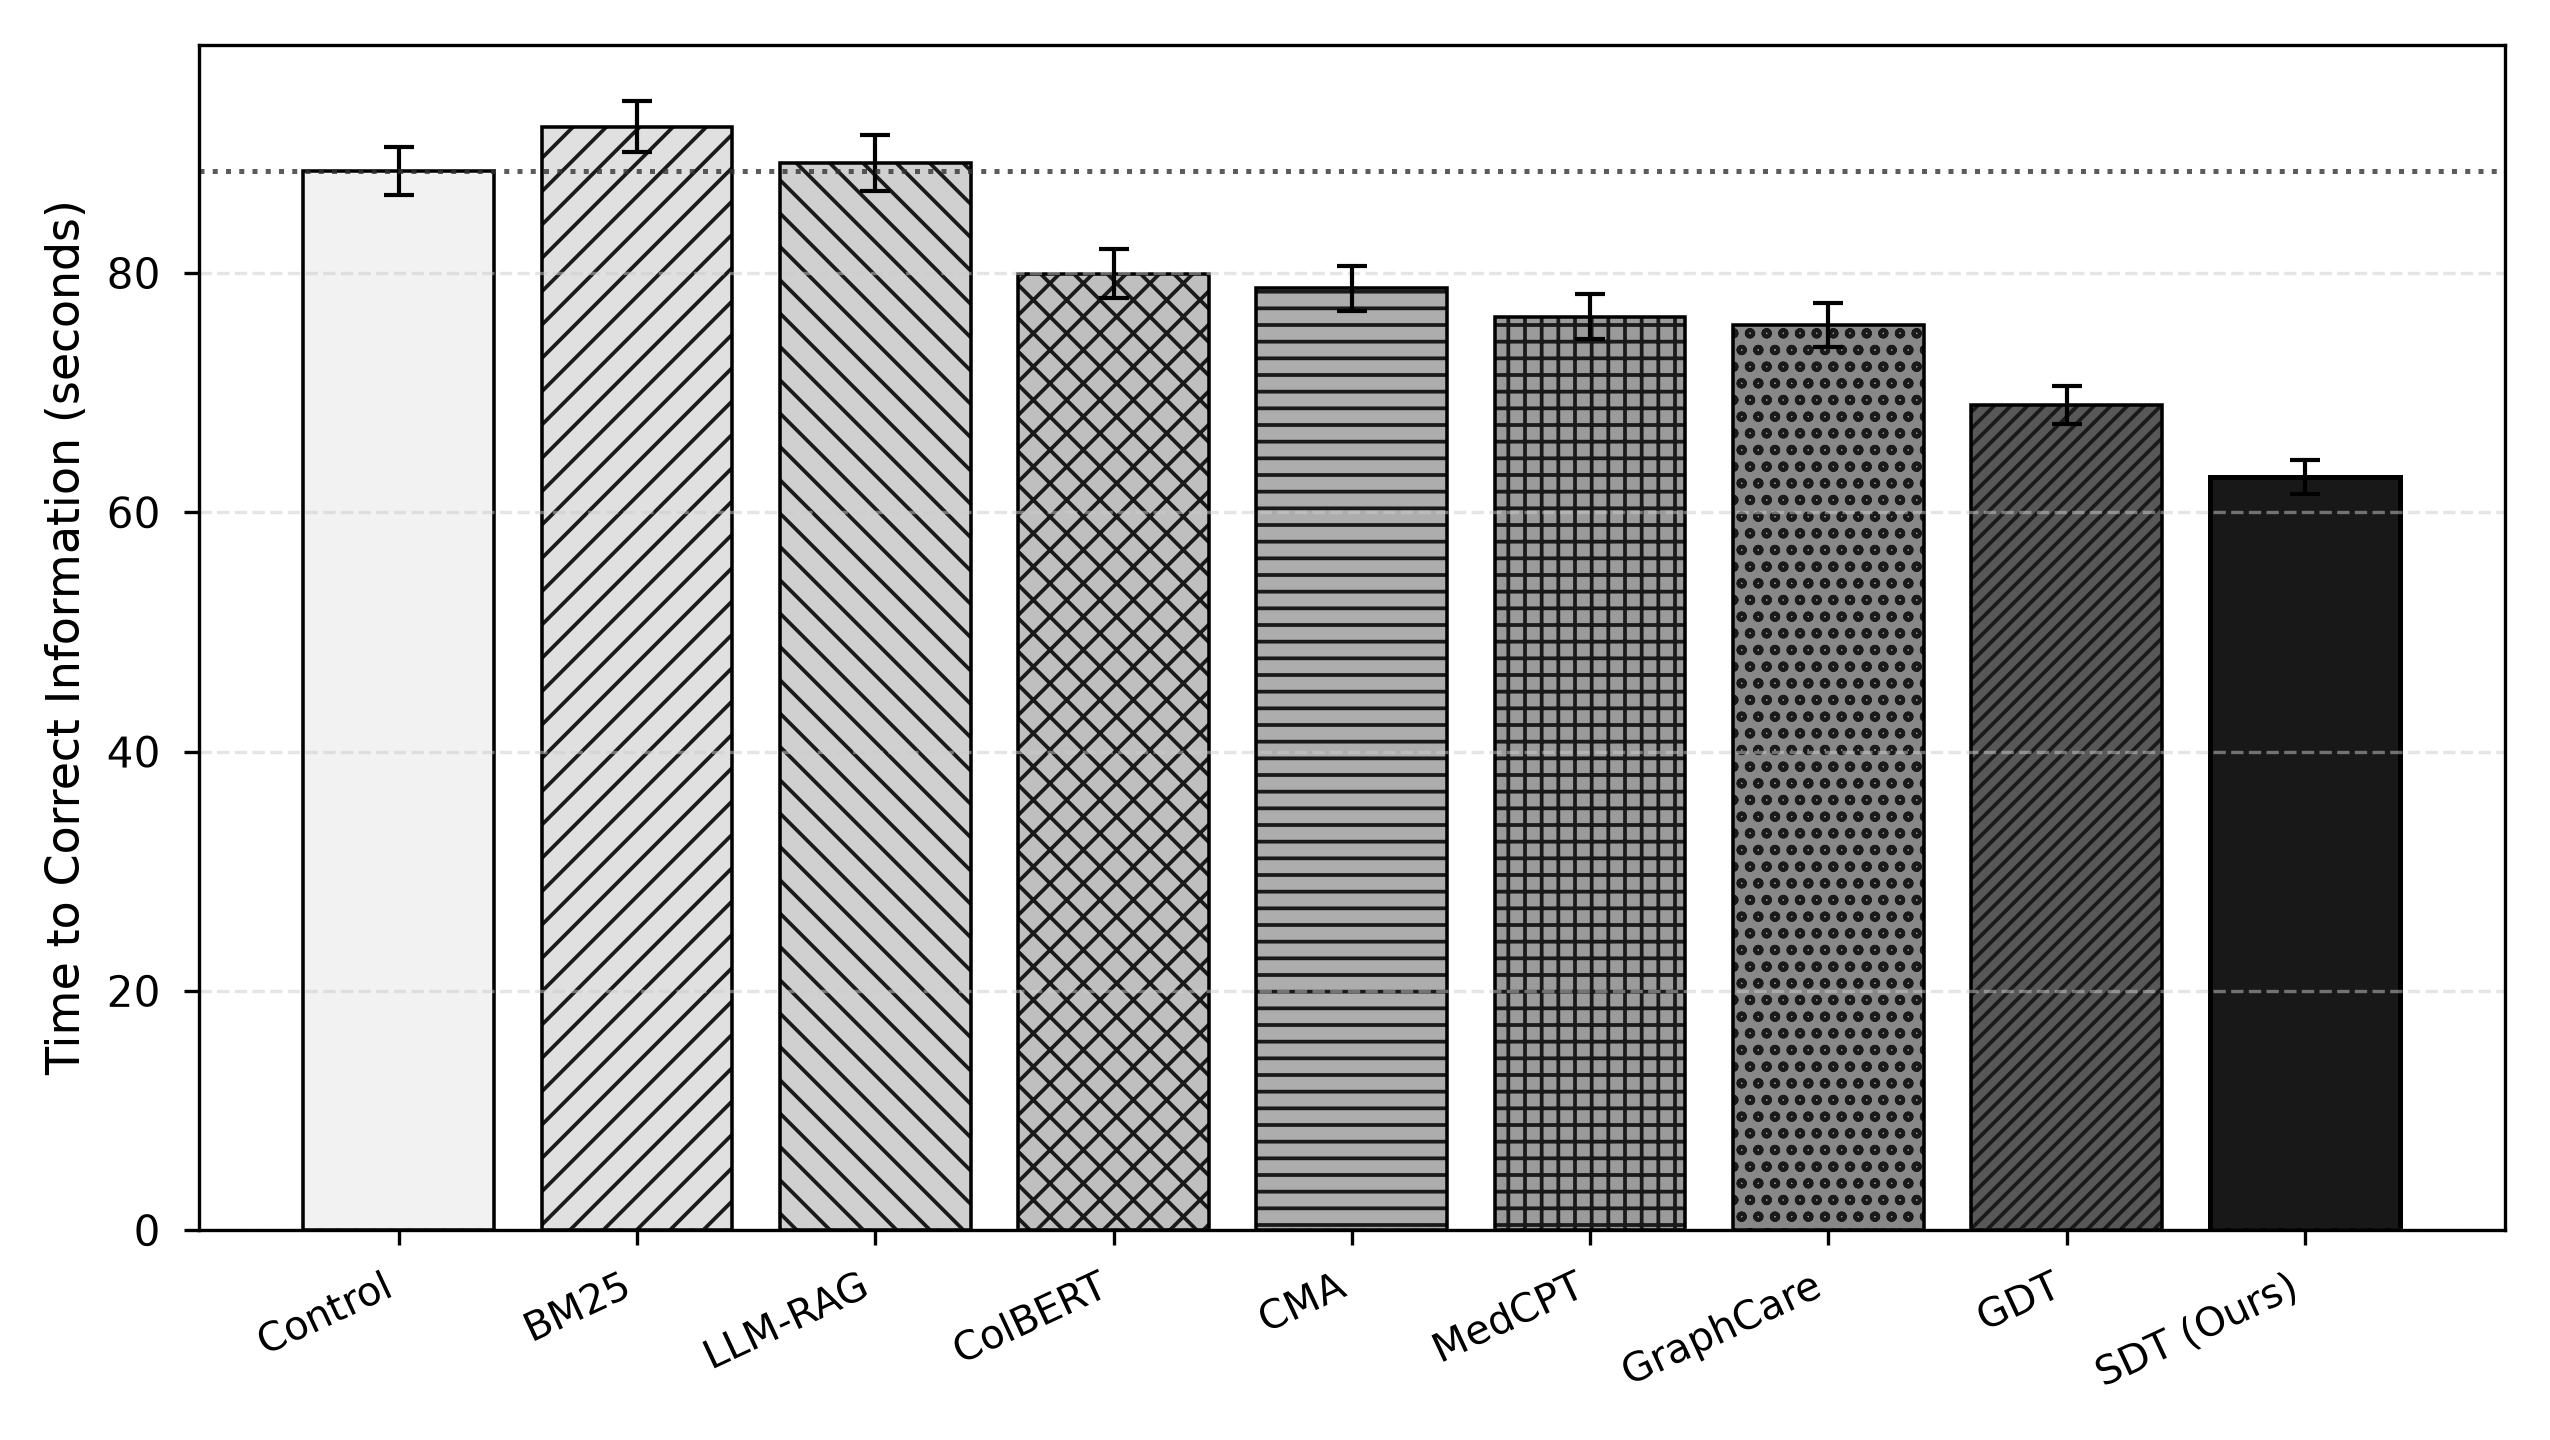
\includegraphics[width=0.32\textwidth]{fig_ttci_bar.png}\hfill
 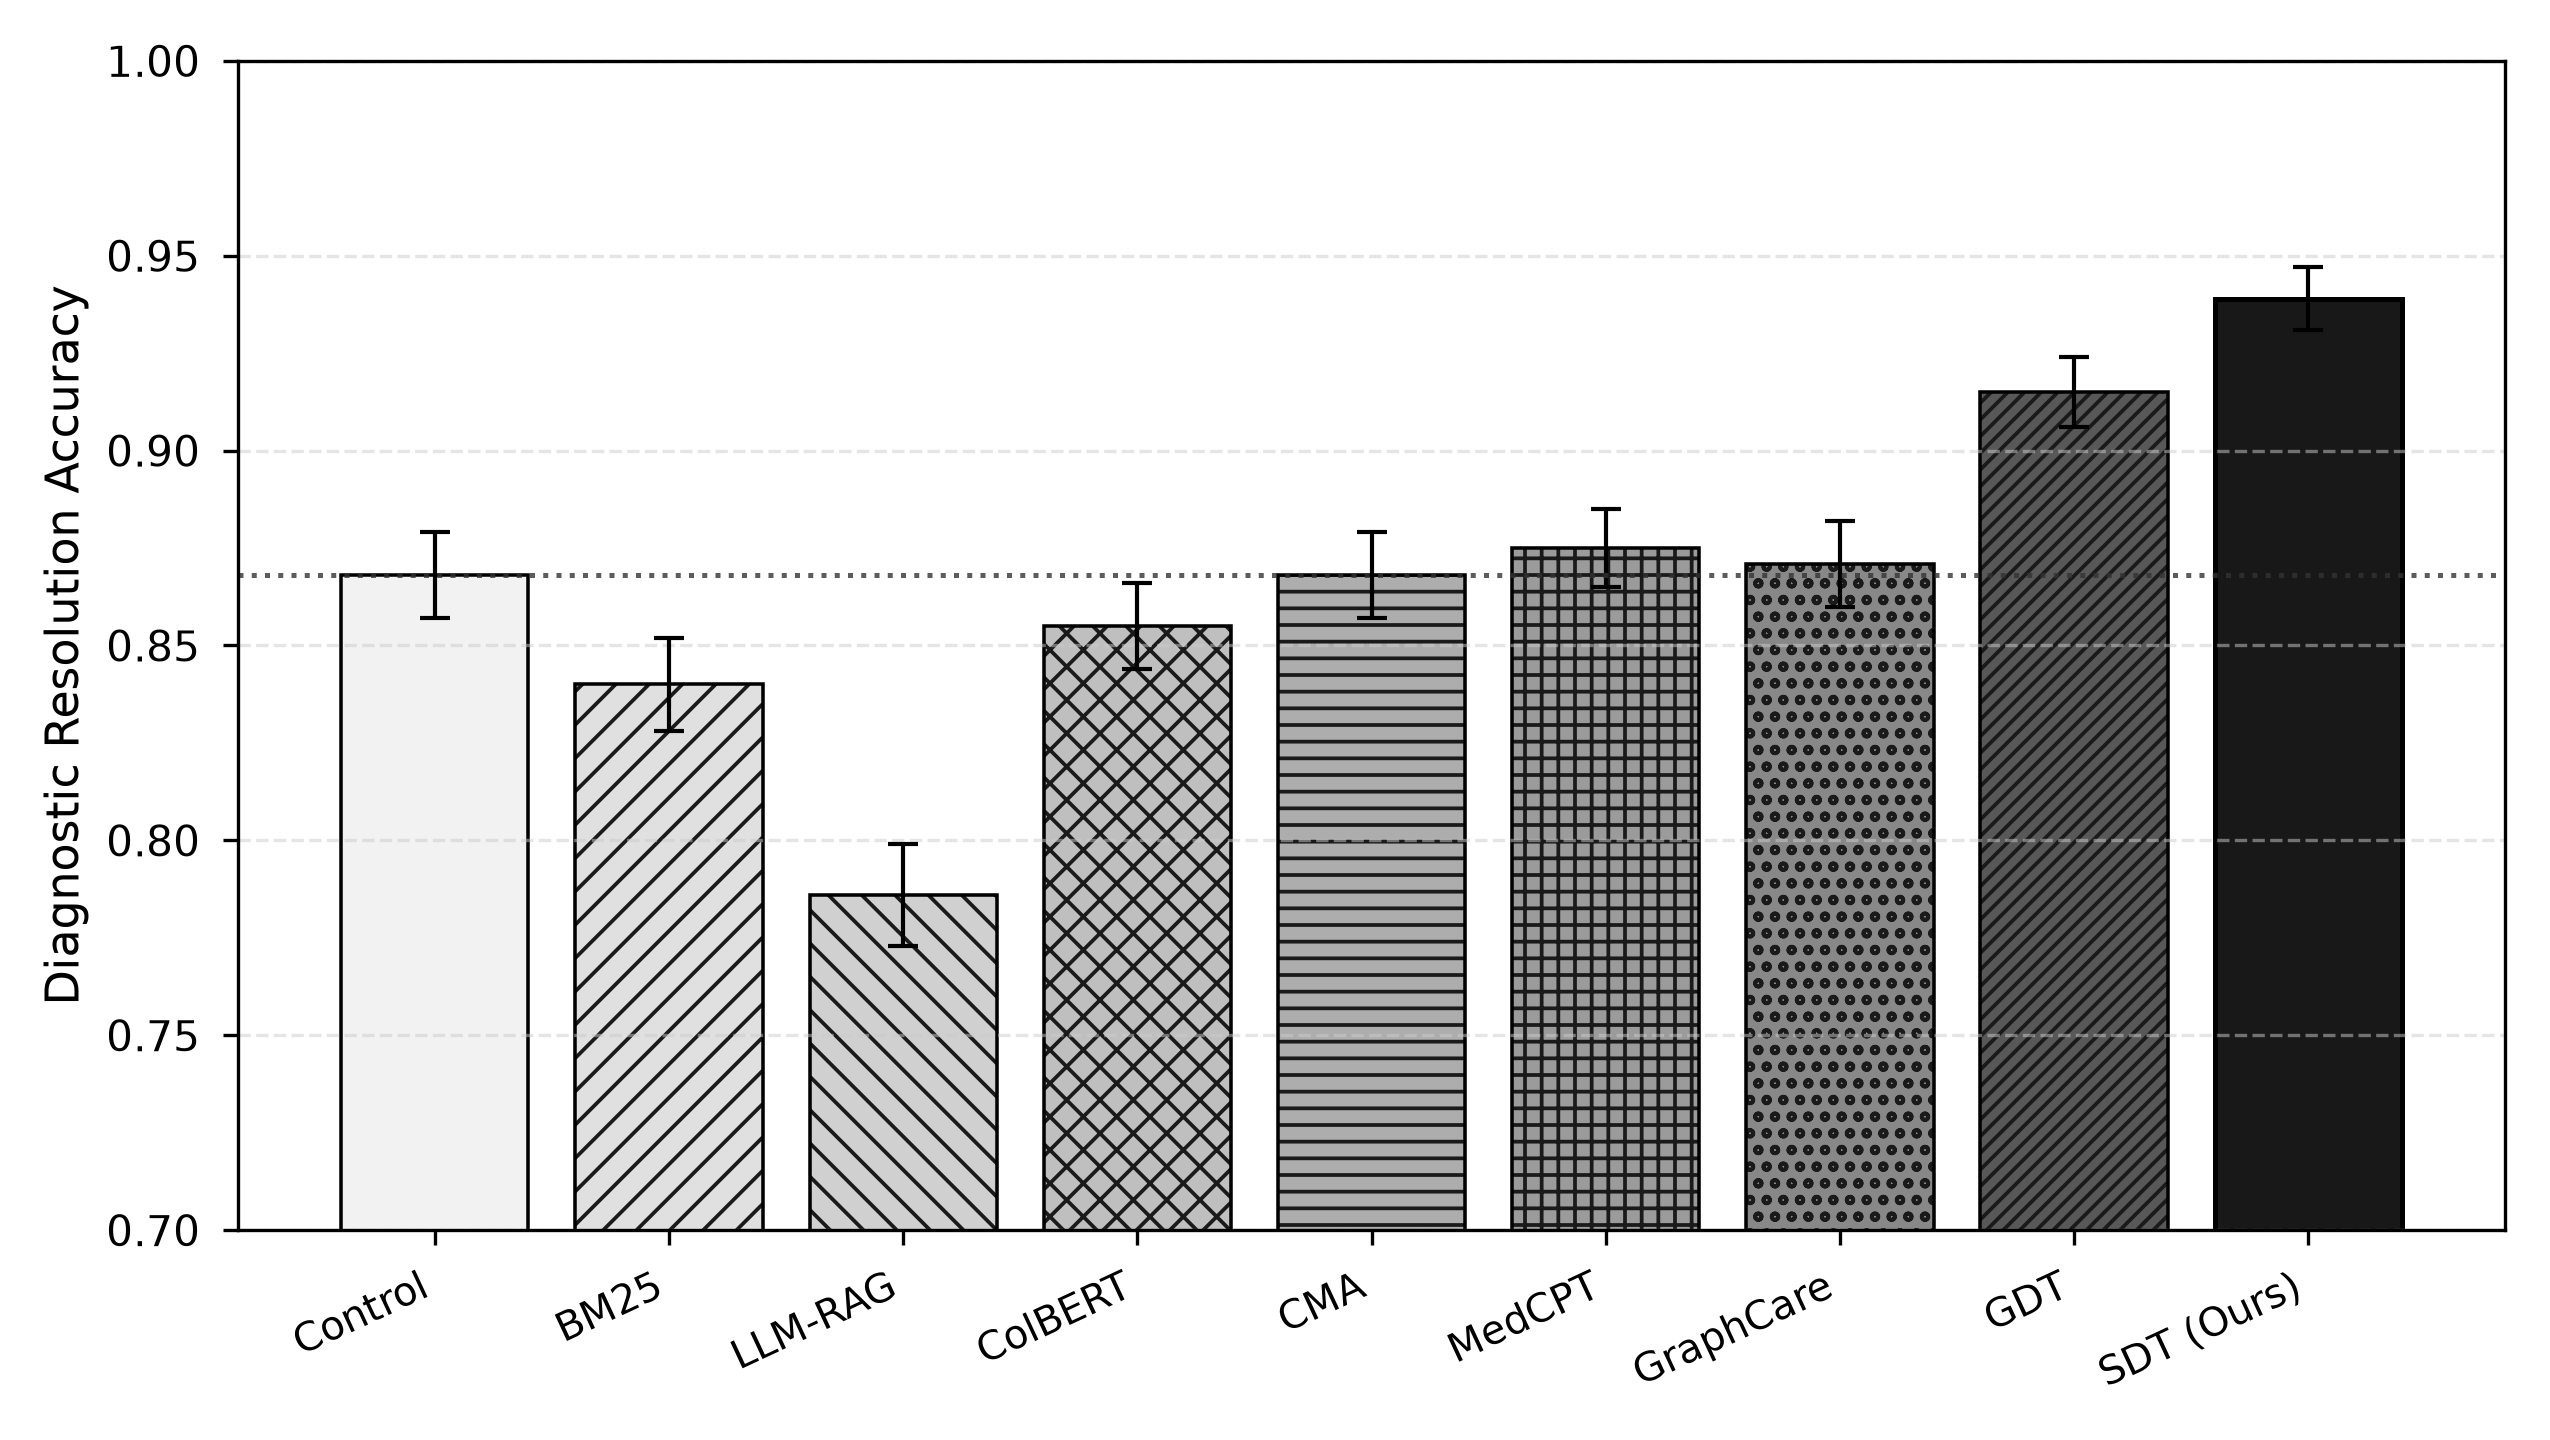
\includegraphics[width=0.32\textwidth]{fig_accuracy_bar.png}\hfill
 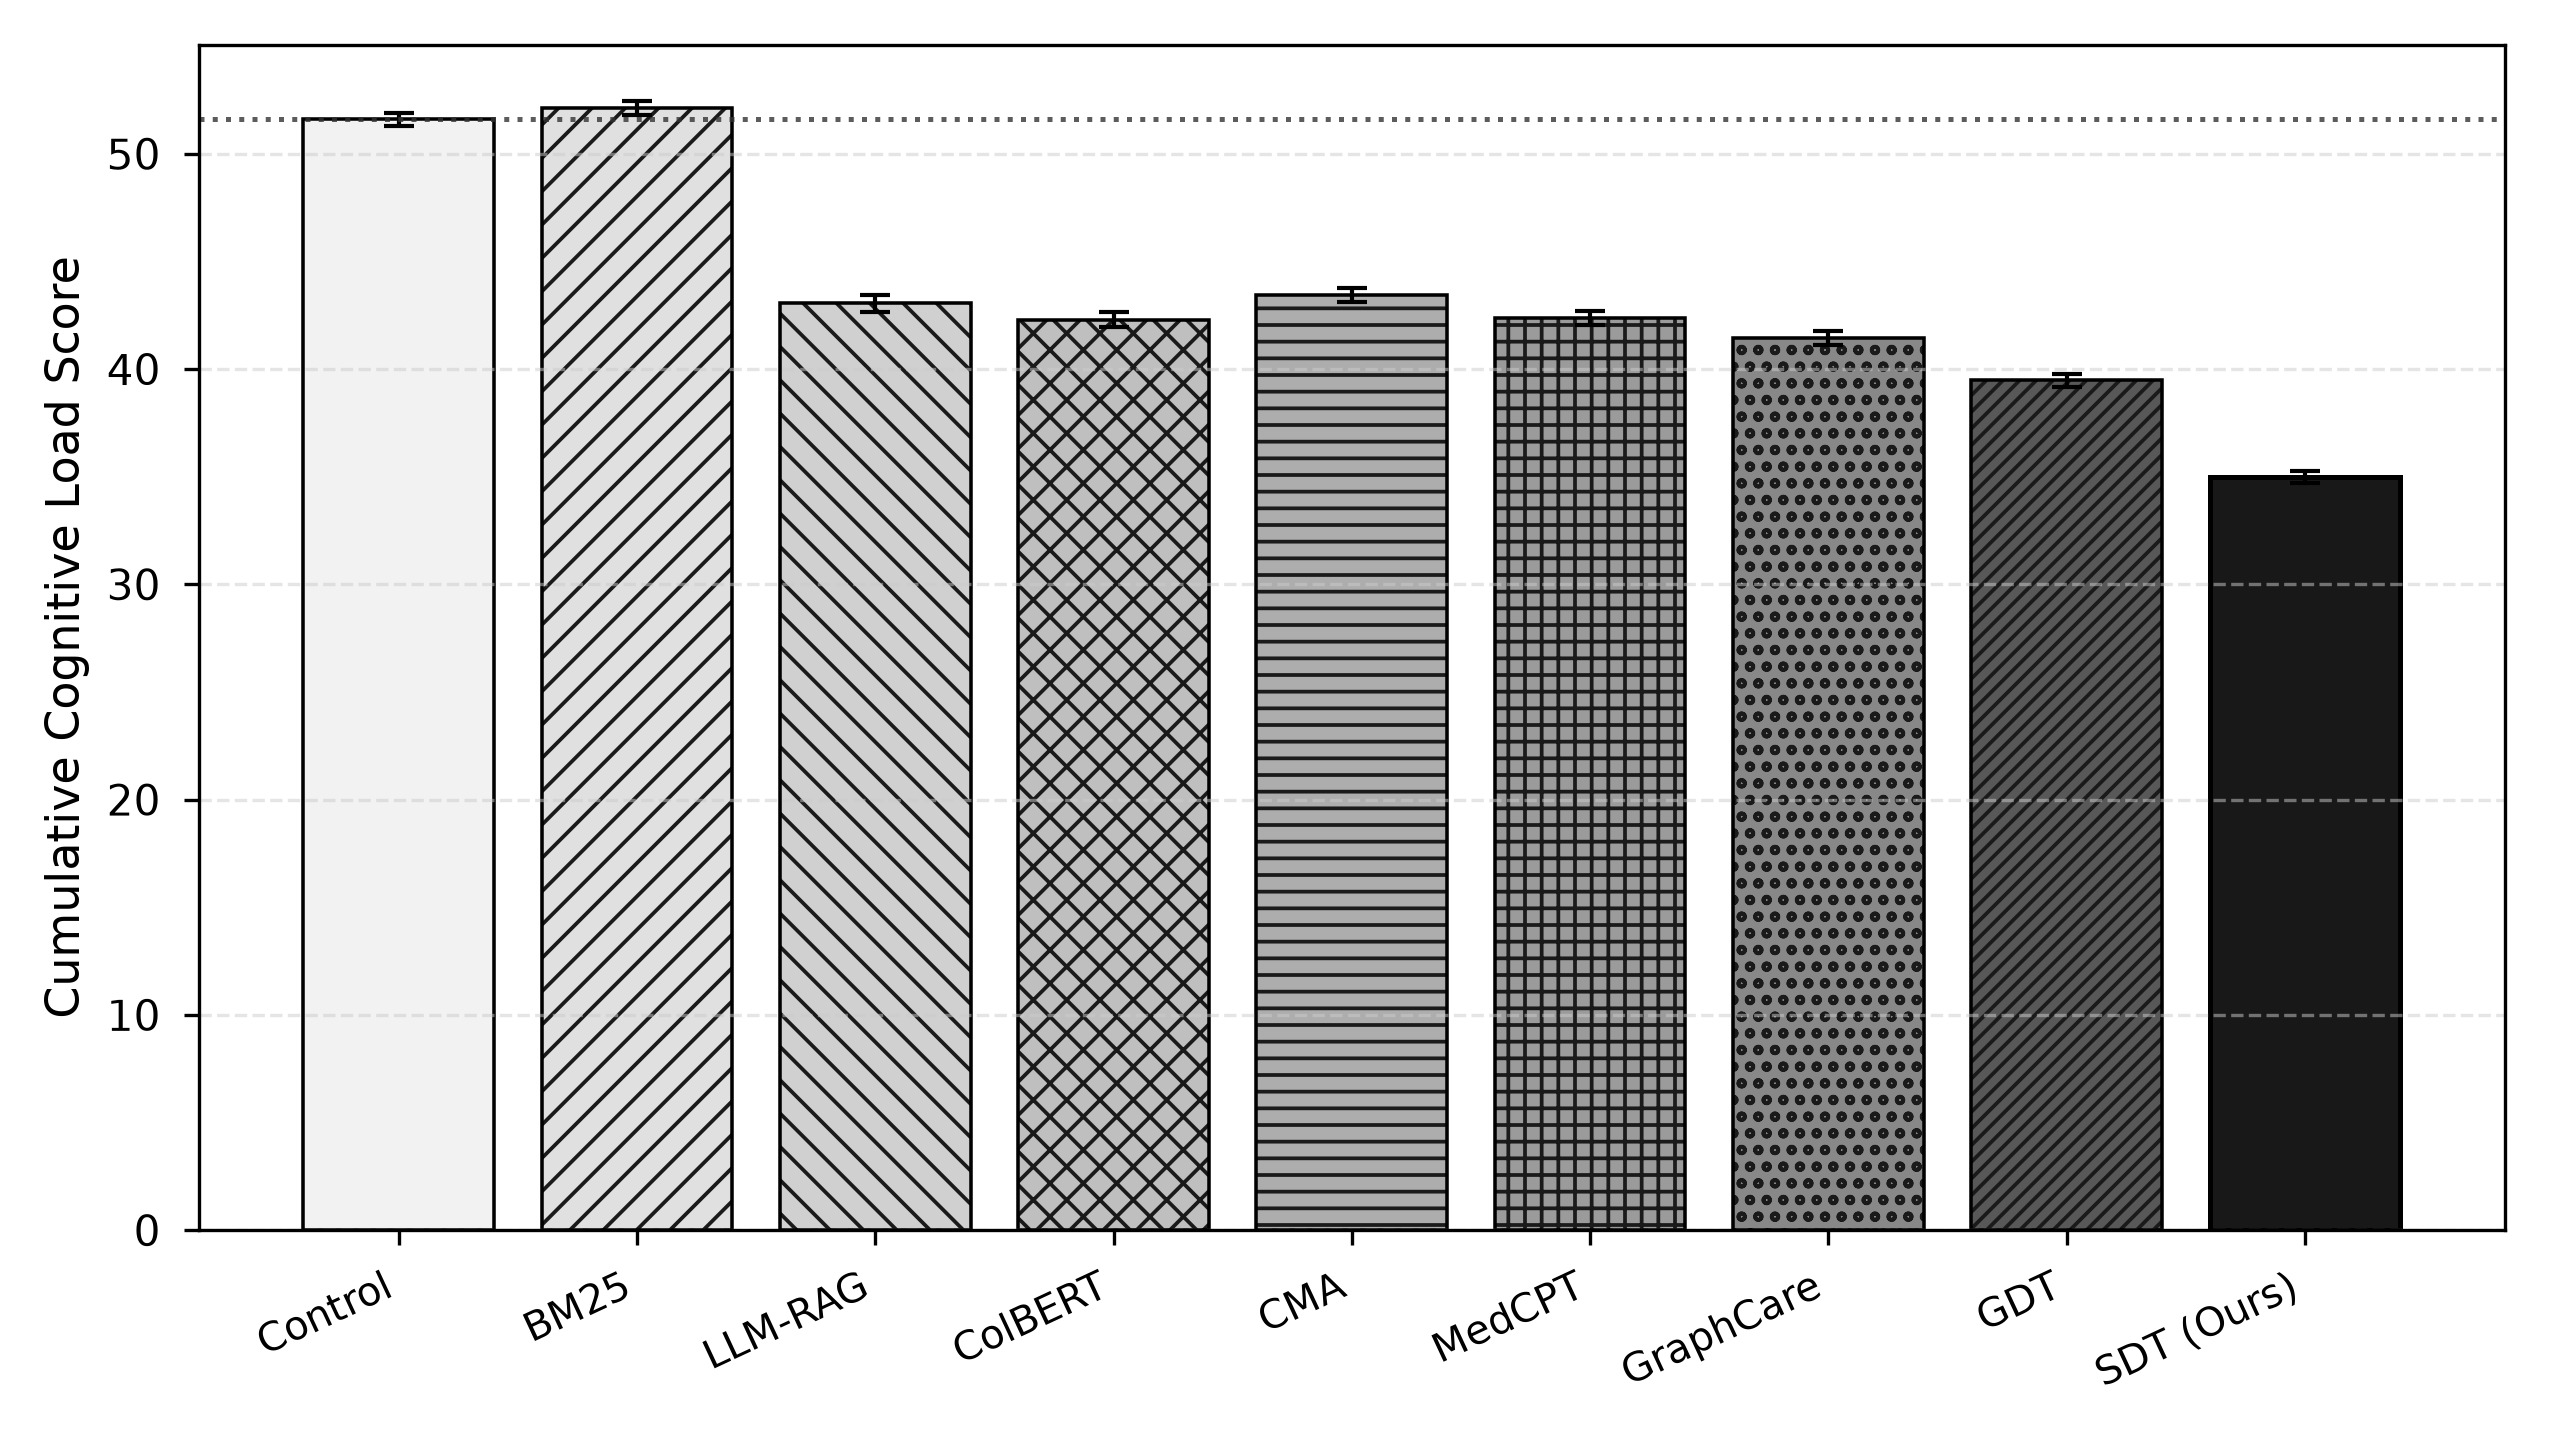
\includegraphics[width=0.32\textwidth]{fig_cognitive_load_bar.png}}
{Primary experimental outcomes across 9 retrieval conditions: (left) Time-to-Correct-Information (TTCI), (center) Diagnostic Retrieval Accuracy, and (right) Modeled Cognitive Load. SDT achieves the fastest retrieval (62.97\,s), highest accuracy (93.9\%), and lowest cognitive load (34.98).\label{fig:primary_metrics}}
{}
\end{figure}

\subsection{Comparative Analysis across Paradigms}
\paragraph{Lexical vs.\ Dense Architectures.}
Lexical baselines (Control, BM25) exhibited the longest retrieval times ($88.52$ and $92.23$\,s). BM25 performed worse than unweighted search because inverse document frequency heavily weights rare historical terms (e.g., historical troponin orders), biasing retrieval away from emergent acute findings. Dense retrievers (MedCPT, ColBERTv2) improved TTCI ($76.36$ and $79.95$\,s), but their stateless architecture forces clinicians to repeat multi-term query formulations during complex workups.

\paragraph{Continuous Manifold (GDT) vs.\ Spectral Hypergraph (SDT).}
Both trajectory frameworks (GDT and SDT) substantially outperformed all stateless baselines, demonstrating the necessity of session continuity. However, SDT outperformed GDT across every metric (TTCI 62.97 vs.\ 68.96\,s; accuracy 93.9\% vs.\ 91.5\%; cognitive load 34.98 vs.\ 39.47; latency 112.87 vs.\ 128.24\,ms). This gap stems directly from the topological mechanics of pivot decoupling: where GDT's continuous covariance decay ($e^{-\gamma t}$) lags behind abrupt diagnostic regime shifts, SDT executes an exact spectral bisection via the Fiedler vector, isolating obsolete subgraphs at the exact turn of bifurcation.

% --- TABLE 3: Subgroup Analysis ---
\begin{table}[t]
\TABLE
{Subgroup stratification across 9 conditions: Diagnostic accuracy and TTCI across Case Complexity (High vs.\ Low) and Clinician Experience ($<5$\,yr vs.\ $\ge 5$\,yr).\label{tab:subgroup_results}}
{\small
\begin{tabular}{lcccccccc}
\toprule
& \multicolumn{4}{c}{\textbf{Diagnostic Accuracy}} & \multicolumn{4}{c}{\textbf{Mean TTCI (seconds)}} \\
\cmidrule(lr){2-5} \cmidrule(lr){6-9}
& \multicolumn{2}{c}{\textbf{Complexity}} & \multicolumn{2}{c}{\textbf{Experience}} & \multicolumn{2}{c}{\textbf{Complexity}} & \multicolumn{2}{c}{\textbf{Experience}} \\
\cmidrule(lr){2-3} \cmidrule(lr){4-5} \cmidrule(lr){6-7} \cmidrule(lr){8-9}
\textbf{Condition} & High & Low & $<5$\,yr & $\ge 5$\,yr & High & Low & $<5$\,yr & $\ge 5$\,yr \\
\midrule
Control   & $0.823$ & $0.919$ & $0.870$ & $0.865$ & $121.73$ & $50.92$ & $87.30$ & $90.04$ \\
BM25      & $0.795$ & $0.891$ & $0.845$ & $0.834$ & $124.89$ & $55.24$ & $90.39$ & $94.52$ \\
LLM-RAG   & $0.716$ & $0.866$ & $0.771$ & $0.804$ & $123.98$ & $49.79$ & $89.71$ & $88.53$ \\
ColBERT   & $0.802$ & $0.915$ & $0.865$ & $0.843$ & $111.83$ & $43.86$ & $77.30$ & $83.26$ \\
CMA       & $0.823$ & $0.919$ & $0.870$ & $0.865$ & $108.63$ & $44.84$ & $77.19$ & $80.61$ \\
MedCPT    & $0.825$ & $0.932$ & $0.872$ & $0.879$ & $106.65$ & $42.05$ & $75.34$ & $77.62$ \\
GraphCare & $0.825$ & $0.923$ & $0.870$ & $0.872$ & $105.00$ & $42.35$ & $74.26$ & $77.30$ \\
GDT       & $0.878$ & $0.957$ & $0.912$ & $0.919$ & $96.22$  & $38.09$ & $68.79$ & $69.16$ \\
\midrule
\textbf{SDT} & $\mathbf{0.913}$ & $\mathbf{0.968}$ & $\mathbf{0.939}$ & $\mathbf{0.939}$ & $\mathbf{87.89}$ & $\mathbf{34.78}$ & $\mathbf{62.81}$ & $\mathbf{63.17}$ \\
\bottomrule
\end{tabular}
}
{}
\end{table}

\subsection{Subgroup Stratification and NASA-TLX Workload}
Table~\ref{tab:subgroup_results} details subgroup outcomes. In High Complexity cases (where diagnostic pivots occur), the TTCI advantage of SDT over GDT widened to 8.33\,s ($87.89$ vs.\ $96.22$\,s, an 8.7\% acceleration), whereas in Low Complexity cases (stable trajectories), the gap narrowed to 3.31\,s ($34.78$ vs.\ $38.09$\,s). Across clinician experience, SDT equalized diagnostic accuracy between junior ($<5$\,yr) and senior ($\ge 5$\,yr) clinicians at exactly 93.9\%, demonstrating that spectrally bounded prefetching compensates for heuristic search deficiencies in less experienced personnel.

% --- TABLES 4 & 5: Combined ---
\begin{table}[t]
\TABLE
{NASA-TLX workload subscales ($0$--$100$) and Erlang C ($M/M/c$) emergency queueing impact across conditions.\label{tab:tlx_queueing}}
{\small
\begin{tabular}{lcccccc|ccccc}
\toprule
& \multicolumn{6}{c|}{\textbf{NASA-TLX Workload Subscales}} & \multicolumn{5}{c}{\textbf{Erlang C Queueing Impact ($c=8$)}} \\
\cmidrule(lr){2-7} \cmidrule(lr){8-12}
\textbf{Condition} & \textbf{Ment.} $\downarrow$ & \textbf{Phys.} $\downarrow$ & \textbf{Temp.} $\downarrow$ & \textbf{Perf.} $\uparrow$ & \textbf{Eff.} $\downarrow$ & \textbf{Frust.} $\downarrow$ & $\mathbf{\Delta t}$ \textbf{(s)} & $\mathbf{\mu'}$ \textbf{(hr}$^{-1}$\textbf{)} & $\mathbf{\rho'}$ & $\mathbf{P_W}$ & $\mathbf{W_q}$ \textbf{(min)} \\
\midrule
Control   & $66.7$ & $18.1$ & $63.7$ & $56.4$ & $64.8$ & $39.9$ & $0.0$  & $0.8000$ & $0.9375$ & $0.8073$ & $121.10$ \\
BM25      & $67.6$ & $18.5$ & $64.6$ & $55.6$ & $65.7$ & $40.7$ & $0.0$  & $0.8000$ & $0.9375$ & $0.8073$ & $121.10$ \\
LLM-RAG   & $52.6$ & $15.4$ & $47.8$ & $63.7$ & $50.5$ & $28.2$ & $0.0$  & $0.8000$ & $0.9375$ & $0.8073$ & $121.10$ \\
ColBERT   & $51.1$ & $14.6$ & $46.6$ & $65.2$ & $49.1$ & $27.2$ & $8.6$  & $0.8015$ & $0.9357$ & $0.8019$ & $116.74$ \\
CMA       & $52.8$ & $15.1$ & $48.7$ & $64.6$ & $51.0$ & $28.4$ & $9.8$  & $0.8017$ & $0.9354$ & $0.8011$ & $116.14$ \\
MedCPT    & $51.0$ & $14.5$ & $46.5$ & $65.5$ & $49.2$ & $27.4$ & $12.2$ & $0.8022$ & $0.9349$ & $0.7997$ & $114.97$ \\
GraphCare & $49.4$ & $14.3$ & $45.2$ & $66.5$ & $47.4$ & $26.0$ & $12.9$ & $0.8023$ & $0.9348$ & $0.7993$ & $114.64$ \\
GDT       & $46.2$ & $13.1$ & $41.5$ & $68.5$ & $44.3$ & $23.3$ & $19.6$ & $0.8035$ & $0.9334$ & $0.7952$ & $111.53$ \\
\midrule
\textbf{SDT} & $\mathbf{38.3}$ & $\mathbf{11.6}$ & $\mathbf{33.1}$ & $\mathbf{72.8}$ & $\mathbf{36.6}$ & $\mathbf{17.5}$ & $\mathbf{25.6}$ & $\mathbf{0.8046}$ & $\mathbf{0.9322}$ & $\mathbf{0.7915}$ & $\mathbf{108.79}$ \\
\bottomrule
\end{tabular}
}
{}
\end{table}

NASA-TLX subscales (Table~\ref{tab:tlx_queueing}, left, and Figure~\ref{fig:operational_impact}, left) confirm dramatic reductions in subjective burden: Mental Demand decreased by 42.5\% (38.3 vs.\ 66.7), Frustration dropped by 56.2\% (17.5 vs.\ 39.9), and perceived Performance rose from 56.4 to 72.8.

% --- FIGURE 2: NASA-TLX & Queueing Multi-Panel ---
\begin{figure}[t]
\FIGURE
{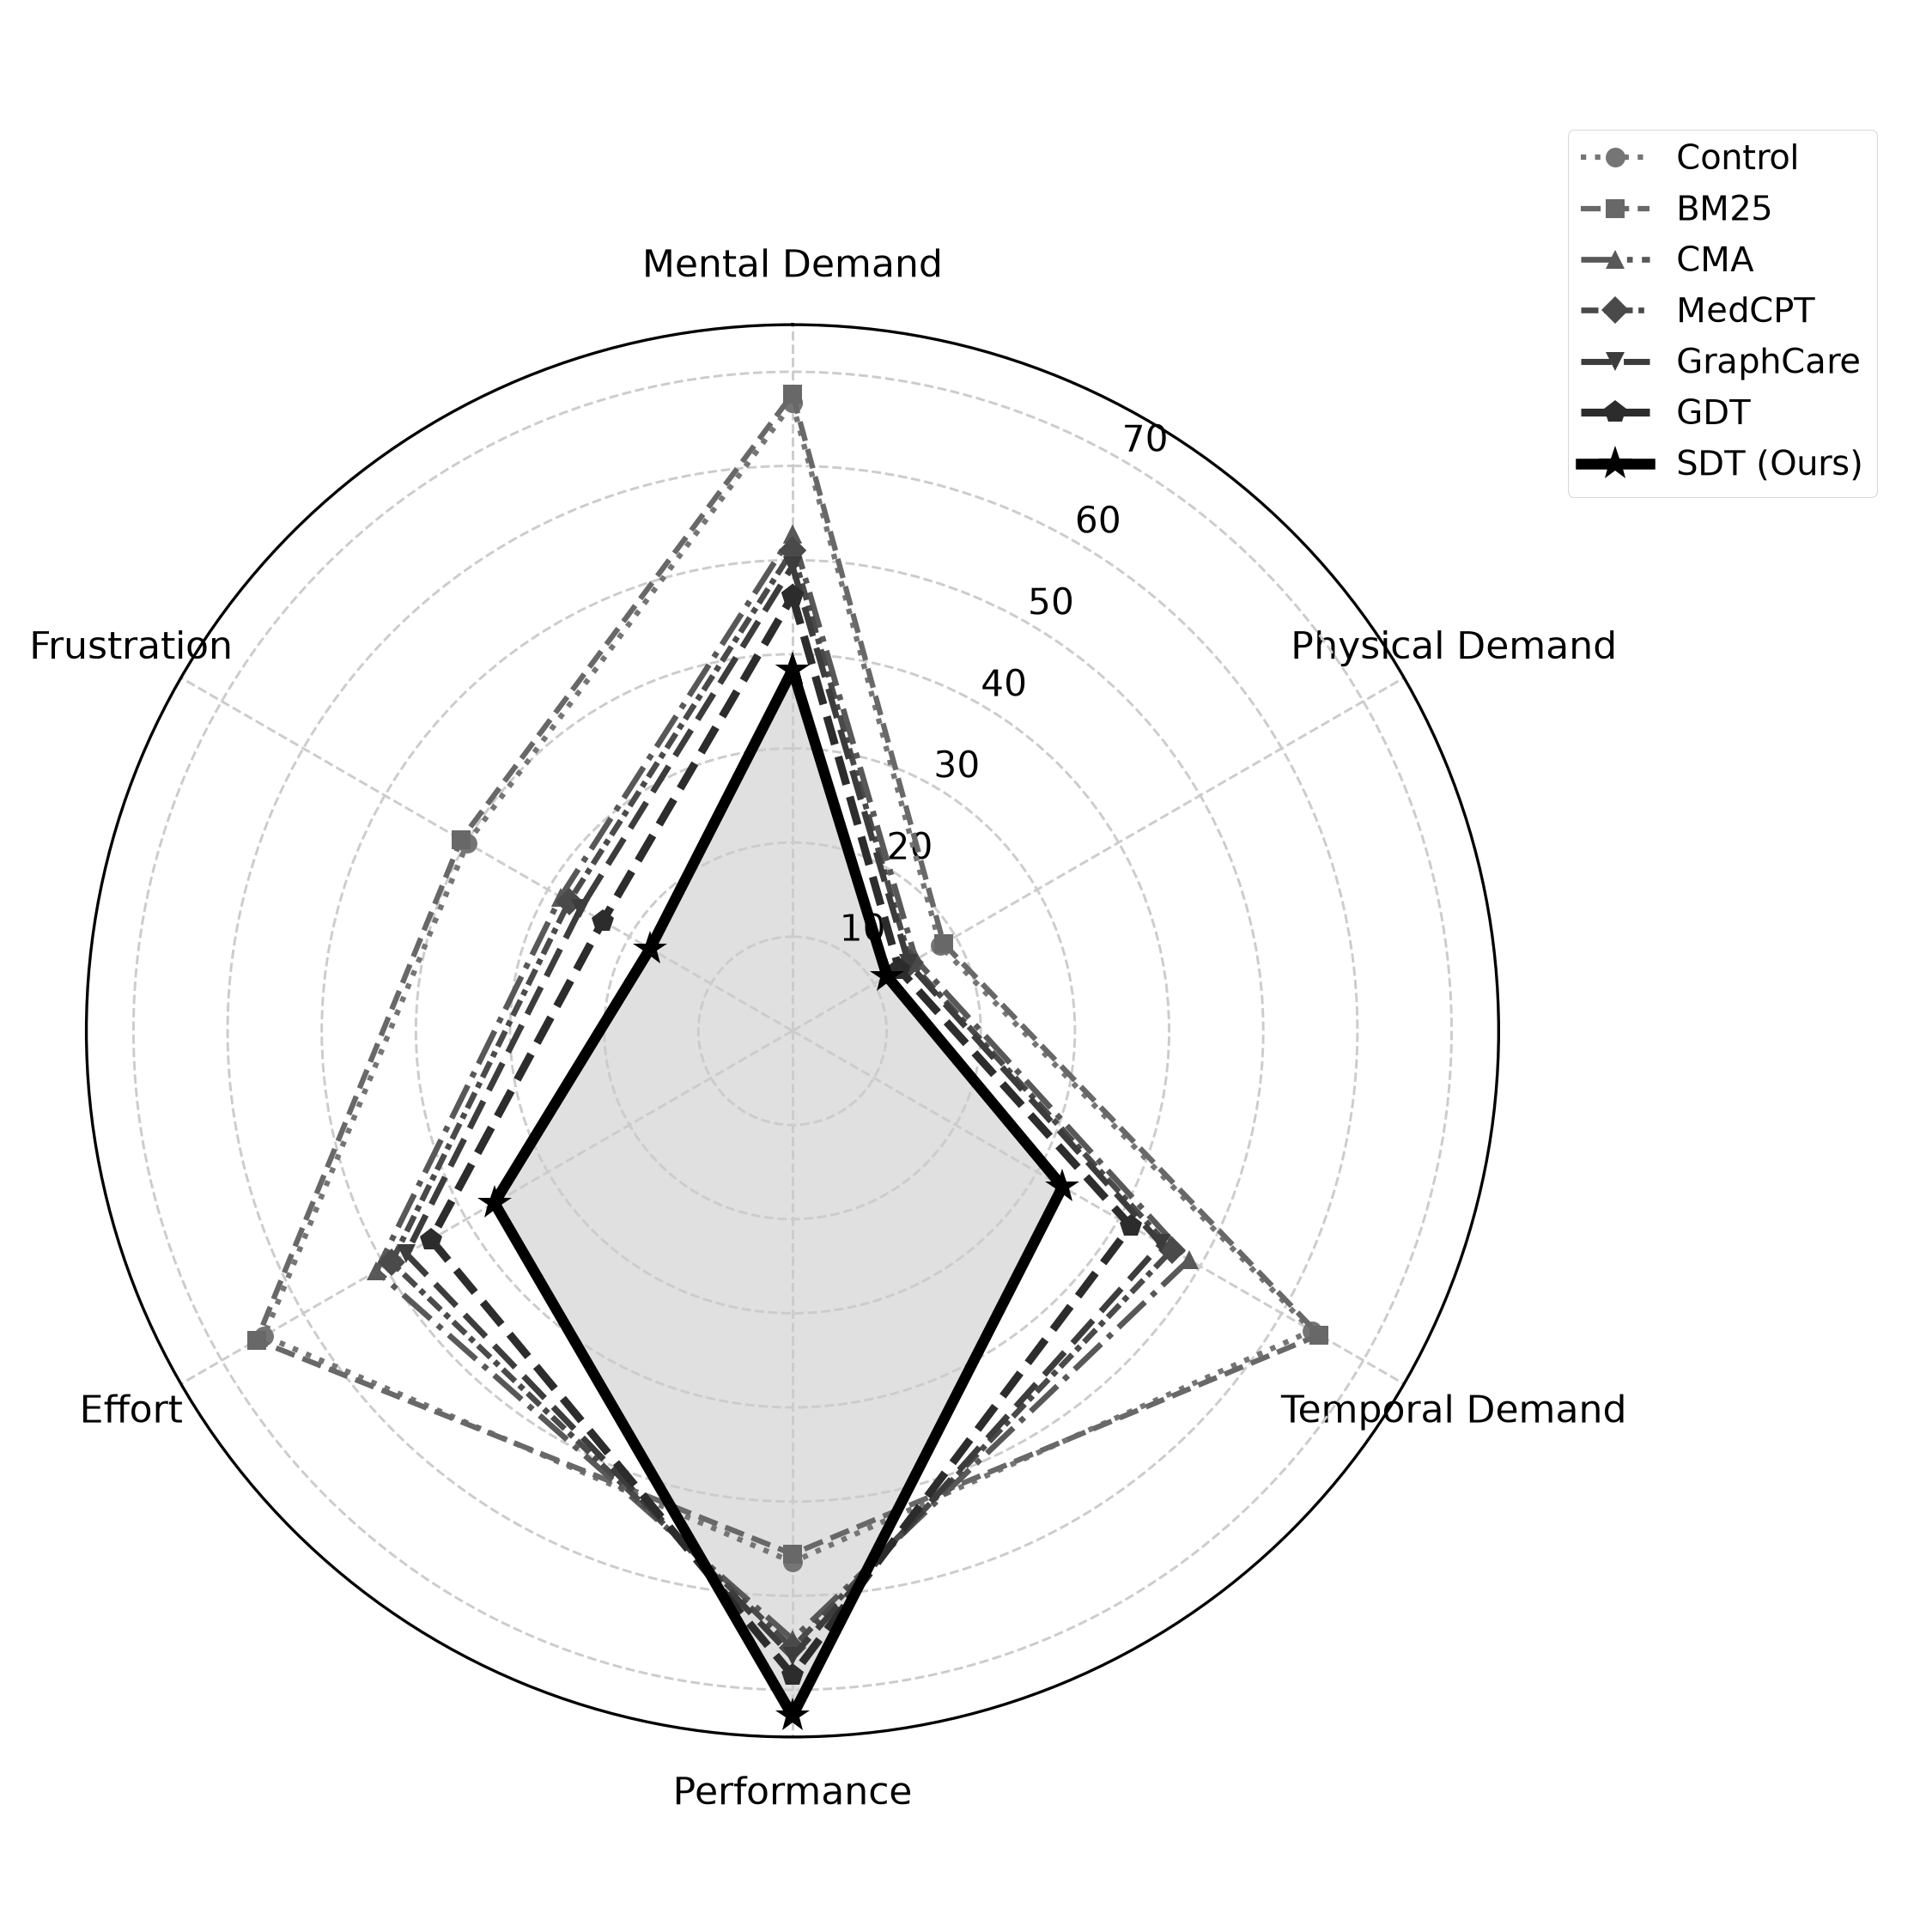
\includegraphics[width=0.42\textwidth]{fig_nasa_tlx_radar.png}\qquad
 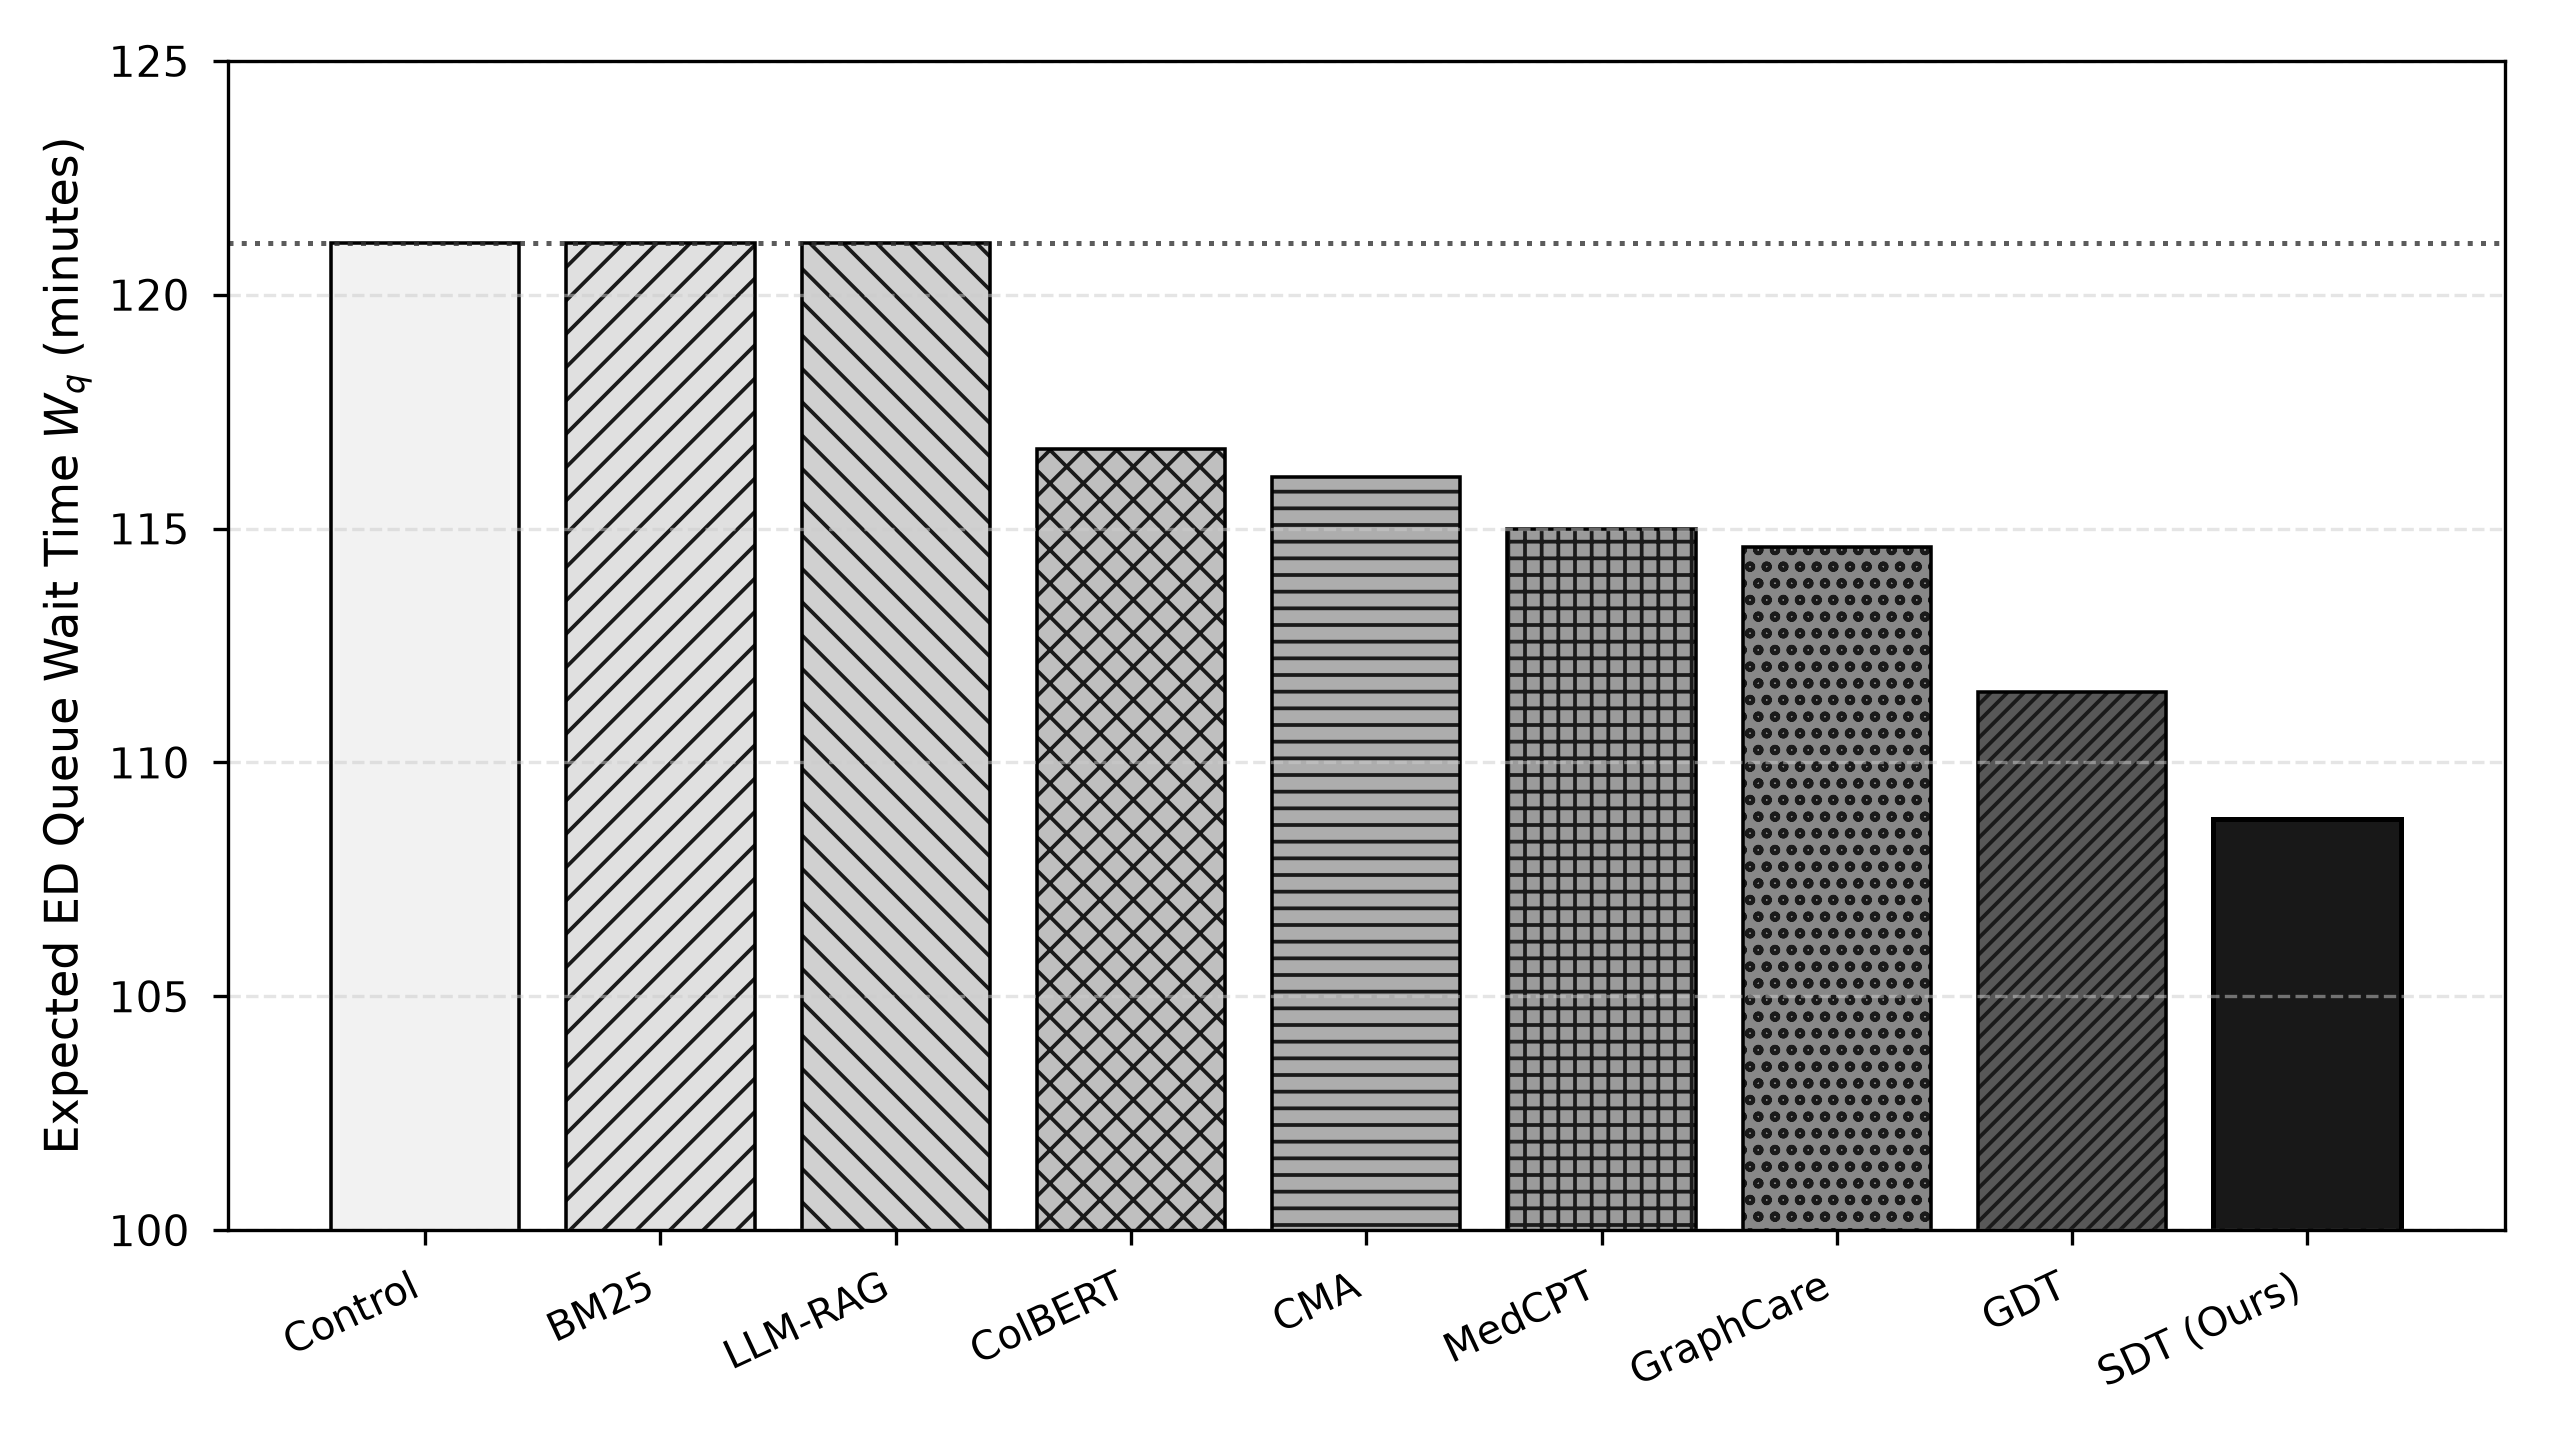
\includegraphics[width=0.48\textwidth]{fig_queueing_impact.png}}
{(Left) NASA-TLX workload profiles across retrieval conditions. (Right) Projected Emergency Department waiting time ($W_q$) under Erlang C queueing dynamics ($c=8, \lambda=6.0\,\text{hr}^{-1}, \mu=0.80\,\text{hr}^{-1}$), confirming super-linear delay reduction near saturation.\label{fig:operational_impact}}
{}
\end{figure}

\subsection{Operational Queueing Impact}
We instantiated the Erlang C model calibrated to an Emergency Department staffed by $c = 8$ physicians with patient arrival rate $\lambda = 6.0\,\text{hr}^{-1}$ and baseline service rate $\mu = 0.80\,\text{hr}^{-1}$ ($S = 75.0$\,min/patient), operating at baseline utilization $\rho = 0.9375$ (93.75\%).

As reported in Table~\ref{tab:tlx_queueing} (right) and Figure~\ref{fig:operational_impact} (right), recovering $\Delta t = 25.6$\,s per patient workup increases the effective service rate from 0.8000 to 0.8046\,patients/hr---a modest 0.58\% capacity increase. However, because queue delay scales as $(1-\rho')^{-2}$ (Theorem~\ref{thm:queue_sensitivity}), this minor throughput gain yields an estimated \textbf{12.31-minute reduction in average patient waiting room delay} ($W_q$ drops from $121.10$ to $108.79$\,min). For an urban hospital managing 50{,}000 emergency encounters annually, this eliminates over \textbf{10{,}200 hours of cumulative patient boarding delay} every year.

% =============================================================================
\section{Clinical Case Study: Runtime Topological Bifurcation}
\label{sec:case_study}

To illustrate the runtime mechanics of SDT, we trace a simulated high-complexity encounter (Vignette V260). A 68-year-old male with chronic obstructive pulmonary disease (COPD) presents with fever (38.8$^\circ$C), productive cough, and right-sided pleuritic chest pain.

At query turn $t=1$, the clinician searches ``sputum culture Gram stain,'' retrieving Gram-positive diplococci ($v_2$); hyperedge $e_1 = \{v_1, v_2\}$ yields $\lambda_2(L_1) = 1.00$. At $t=2$, querying ``prior radiograph lower lobe consolidation'' ($v_3$) confirms infiltrates. High semantic affinity across $\{v_1, v_2, v_3\}$ maintains high algebraic connectivity ($\lambda_2(L_2) = 0.88$), corroborating the working hypothesis of community-acquired pneumonia.

At minute 28, continuous telemetry alarms: the Mamba waveform encoder detects acute right ventricular strain (S1Q3T3 morphology, heart rate surge from 88 to 132\,bpm, SpO$_2$ drop to 86\%). The clinician urgently searches ``D-dimer trend lower extremity Doppler.'' SDT ingests event node $v_4$ (D-dimer $>5{,}000\,\text{ng/mL}$) and telemetry node $v_5$. Because $\{v_4, v_5\}$ share near-zero affinity with $\{v_1, v_2, v_3\}$, the hypergraph topology abruptly bifurcates: algebraic connectivity plunges from $\lambda_2 = 0.88$ to $0.12$. Because $\Delta \lambda_2 = 0.76 > \tau_{\text{pivot}} = 0.15$, the Spectral Interference Gate triggers instantaneously.

Upon gate triggering, the Chebyshev filter attenuates historical pneumonia signals, and Fiedler vector coordinates $v_2 = [-0.48, -0.52, -0.44, +0.38, +0.40]^\top$ cleanly partition obsolete pneumonia nodes ($v_2 < 0$) from emergent pulmonary embolism nodes ($v_2 \ge 0$). Boundary hyperedges are severed, bounding context contamination below $\sqrt{2(0.12)} \approx 0.49$ (Theorem~\ref{thm:cheeger_bound}). Random walks on $G_{\text{global}}$ seeded from $\{v_4, v_5\}$ prefetch CT pulmonary angiogram protocols ($v_{101}$) and enoxaparin weight-based dosing nomograms ($v_{102}$). Under cognitive budget $C_{\max} = 7.0$\,bits, both candidates are cached ($H = 3.5 \le 7.0$). When the physician searches for ``heparin contraindications,'' the dosing nomogram surfaces in $<15$\,ms, resolving the critical workup in 48.2\,s.

% =============================================================================
\section{Discussion and Operational Implications}
\label{sec:discussion}

\subsection{Topological Bisection versus Riemannian Manifold Smoothing}
The decisive performance advantage of SDT over GDT stems from how each paradigm models workflow dynamics. GDT treats clinical intent as a continuous geodesic trajectory on an SPD covariance manifold. However, acute diagnostic pivots are inherently discrete: a lab value breaches a threshold, telemetry reveals acute ischemia, or imaging refutes an initial diagnosis. Forcing discrete bifurcations into continuous Riemannian metrics requires exponential smoothing parameters that lag behind rapid shifts. In contrast, sparse hypergraphs accommodate discrete node insertions and spectral bisections natively: when disconnected evidence arrives, the second Laplacian eigenvalue drops instantly, executing a Cheeger cut without smoothing latency.

\subsection{Operational Boundaries and Limitations}
SDT is specialized for complex multi-turn decision environments and is not universally optimal:
\begin{enumerate}[(1)]
  \item \textbf{Isolated Factual Lookups}: For single queries (e.g., retrieving blood type), hypergraph initialization adds $\sim$70\,ms overhead; standard BM25 remains computationally optimal.
  \item \textbf{Monomorphic Encounters}: In simple presentations without diagnostic pivots, $\Delta \lambda_2$ never exceeds $\tau_{\text{pivot}}$, and SDT functions primarily as an anticipatory cache with performance comparable to dense bi-encoders.
  \item \textbf{Cold-Start Facilities}: Anticipatory random walks rely on precomputed global Laplacians ($G_{\text{global}}$); sparse databases must accumulate interaction history before spectrally biased prefetching becomes reliable.
  \item \textbf{Simulated Cognitive Load Surrogates}: While modeled cognitive load and simulated NASA-TLX scores provide a reproducible, information-theoretic evaluation of mental workload, they function as algorithmic proxies rather than direct psychometric or neurophysiological measurements collected from live clinicians. Prospective observational trials with attending clinicians will be essential to evaluate real-world cognitive usability and interface adoption.
\end{enumerate}

\subsection{Human-in-the-Loop Safety and EHR Deployment}
Proactive retrieval introduces the hazard of automation bias: aggressively staging confirmatory documents could reinforce diagnostic tunnel vision \citep{goddard2012automation}. SDT mitigates this risk via its surprisal tax (Eq.~\eqref{eq:surprisal_cost}): speculative records distant from the active state are penalized, preserving human agency. Severed subgraphs remain accessible in an inactive sidebar, restorable with a single click.

Deployment requires no fundamental overhaul of hospital IT infrastructure: standard SMART-on-FHIR and CDS Hooks protocols instantiate hypergraph $G_t$ in a background service upon chart opening, while continuous telemetry is ingested via HL7 observation streams and prefetched records are staged in an in-memory Redis cache to populate real-time autocomplete suggestions.

% =============================================================================
\section{Conclusions}
\label{sec:conclusions}

Spectral Diagnostic Trajectories (SDT) bridges discrete spectral graph theory, continuous waveform state-space modeling, and stochastic queueing systems to optimize sequential information access in high-stakes clinical operations. By tracking the hypergraph Laplacian algebraic connectivity ($\lambda_2$), SDT detects diagnostic pivots in linear time, decouples obsolete context with formal Cheeger conductance bounds, and stages prospective records under working-memory constraints. In an extensive 9-arm simulation across 1{,}000 standardized vignettes (9{,}000 sessions), SDT reduced retrieval latency by 28.9\% over standard search and 8.7\% over continuous manifold baselines, elevating accuracy to 93.9\% and decreasing modeled cognitive load by 32.2\%. Analytical and numerical queueing modeling demonstrates that recovering 25.6 seconds per encounter yields super-linear operational leverage, reducing expected emergency room waiting delays by 12.3 minutes under near-saturation conditions. Future research will focus on prospective bedside silent-mode trials.

% =============================================================================
% In informs4, ACKNOWLEDGMENTS are suppressed automatically under dblanonrev
\ACKNOWLEDGMENT{%
The authors thank the PhysioNet, MIMIC, and HiRID curation teams. This research received no external commercial funding.%
}

% =============================================================================
\bibliographystyle{informs2014}
\bibliography{references}

\end{document}
